
\documentclass[a4paper,11pt]{article}

\usepackage{amsmath}
\usepackage{amssymb}
\usepackage{bm}
\usepackage{caption}
\usepackage{colortbl}
\usepackage{enumitem}
\usepackage{etaremune}
\usepackage{eurosym}
\usepackage{fancyhdr}
\usepackage{geometry}
\usepackage{graphicx}
\usepackage{lineno}
\usepackage{mathtools}
\usepackage{multicol}
\usepackage{multirow}
\usepackage{parskip}
\usepackage{setspace}
\usepackage{subcaption}
\usepackage{tabularx}
\usepackage{tabulary}
\usepackage{titlesec}
\usepackage[T1]{fontenc}
\usepackage{times}
\usepackage{url}
\usepackage{wrapfig}
\usepackage{xcolor}

\usepackage[colorinlistoftodos]{todonotes}

\usepackage{array}
\newcolumntype{C}[1]{>{\centering\arraybackslash}p{#1}}

% Shrink the spacing between references in the bibliography
%\usepackage{etoolbox}
%\patchcmd\thebibliography
% {\labelsep}
% {\labelsep\itemsep=-8pt\relax}
% {}
% {\typeout{Couldn't patch the command}}
 %%% End of code to add %%%

\bibliographystyle{h-physrev}

\renewcommand{\thesection}{\Alph{section}}

\newcounter{bar}
\newcommand{\taskcounter}{%
        \stepcounter{bar}%
        \thebar}

\setlist[itemize]{itemsep=-4pt, topsep=-2pt}

\usepackage{hyperref}

\hypersetup{ colorlinks=false,
		     linkcolor=green,
		     urlbordercolor=blue,
		     pdfborderstyle={/S/U/W 1}}
		     
\renewcommand{\smallskip} {\vspace{0.1in}}
\renewcommand{\medskip}   {\vspace{0.2in}}
\renewcommand{\bigskip}   {\vspace{0.4in}}

\geometry{tmargin=1.5cm, bmargin=1.5cm, lmargin=2cm, rmargin=2cm}

\setlength{\headheight}{15pt} 

\footskip=22pt
\headsep=18pt

\titlespacing*{\section}{0pt}{2pt}{2pt}
\titlespacing*{\subsection}{0pt}{2pt}{2pt}
\titlespacing*{\subsubsection}{0pt}{1pt}{1pt}


\singlespacing
%\linenumbers

%%%%%%%%%%%%%%%%%%%%%%%%%%%%%%%%%%%%%%%%%%%%%%%%%%%%%%%%%%
% Cover Page
%%%%%%%%%%%%%%%%%%%%%%%%%%%%%%%%%%%%%%%%%%%%%%%%%%%%%%%%%%

\begin{document}
\renewcommand{\headrulewidth}{0pt}

% \pagestyle{fancyplain}

% \lhead[\it Koskinen]{\it Koskinen}
% \chead{B1 - Cover Page}
% \rhead{NuUnity}

\vspace{1cm}

\centerline{ \large \textbf{ERC Starting Grant 2021}} \smallskip
\centerline{ \large \textbf {Research Proposal [Part B1]}} \smallskip

\vspace{1.0cm}

%
\centerline{\huge \textbf{A wrinkle in space-time}}
\vspace{0.5cm}
\centerline{ \huge {\bf (SpWrinkle)}} 


%~\\

\vspace{1.5cm}

\noindent
Cover page: \\
- Principal Investigator: Thomas Simon Stuttard\\
- Host Institution: Niels Bihr Institute, University of Copenhagen\\
- Proposal Duration: $60$ months\\

~\vspace{0. cm}

\noindent
{\bf Proposal Summary}:

Proposal summary (identical to the abstract from the online proposal submission forms, section 1). 

The abstract (summary) should, at a glance, provide the reader with a clear understanding of the objectives of the research proposal and how they will be achieved. The abstract will be used as the short description of your research proposal in the evaluation process and in communications to contact in particular the potential remote referees and/or inform the Commission and/or the programme management committees and/or relevant national funding agencies (provided you give permission to do so where requested in the online proposal submission forms, section 1). It must therefore be short and precise and should not contain confidential information. 

Please use plain typed text, avoiding formulae and other special characters. The abstract must be written in English. There is a limit of 2000 characters (spaces and line breaks included).

%%%%%%%%%%%%%%%%%%%%%%%%%%%%%%%%%%%%%%%%%%%%%%%%%%%%%%%%%%
% Extended Synopsis
%%%%%%%%%%%%%%%%%%%%%%%%%%%%%%%%%%%%%%%%%%%%%%%%%%%%%%%%%%
\newpage

% \lhead[\it Koskinen]{\it Koskinen}
% \chead{B1 - Extended Synopsis}
% \rhead{NuUnity}

%\begin{center}
%  {\LARGE\bf Neutrino Oscillation and Precision Tests of}\\[1ex]
%  {\LARGE\bf Unitarity at the South Pole}\\[1ex]	
%  {\large David Jason Koskinen}\\[1ex]
% \end{center}

\section{Extended Synopsis}
\vspace{0.1 cm}

% \begin{wrapfigure}{R}{0.45\textwidth} %this figure will be at the right
%     \centering
% 		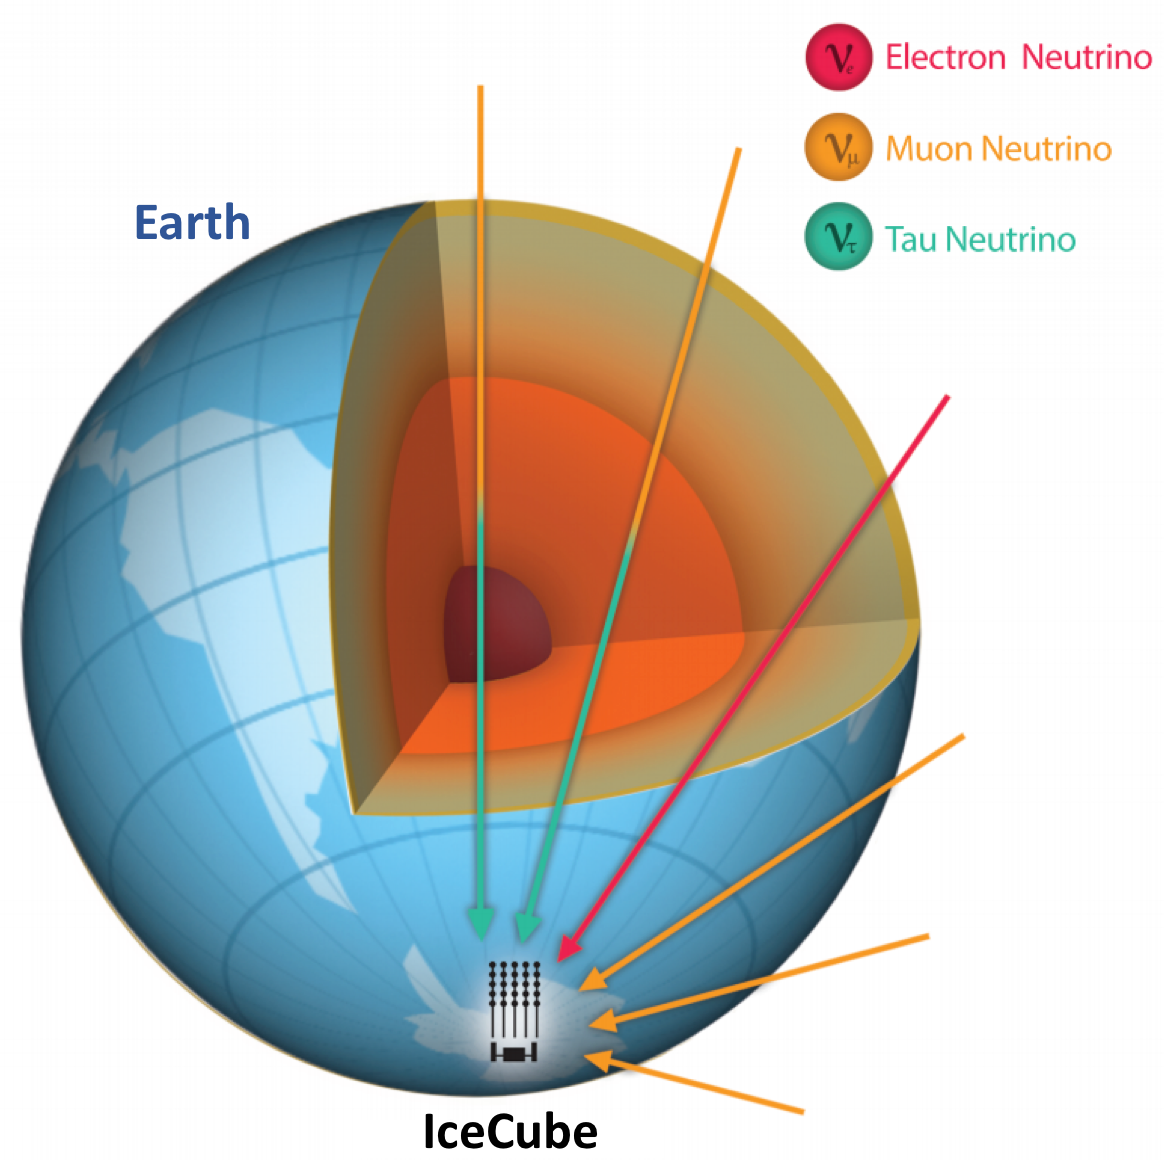
\includegraphics[width=1.\linewidth]{images/atmo_osc.png}
% 		\caption{Neutrinos produced in the atmosphere cross the Earth before detection in IceCube, oscillating and potentially experiencing the influence of quantum gravity as they propagate.}
% 		\vspace{-7pt}
% 		\label{fig:atmo_osc}
% \end{wrapfigure}
\todo{Which figures?}
\todo{Scan through B2 theory section and check if I'm missing any key points}

Despite every other force in Nature being successfully described by quantum mechanics and decades of theoretical efforts, there is currently no quantum theory of gravity. A major contributing factor to this impasse is the paucity of meaningful experimental constraints to guide theory, a consequence of the astounding weakness of gravity whose subatomic effects are expected to be suppressed at the energy and distance scales we can experimentally probe, only becoming large at the \textit{Planck scale} -- $10^{19}$\,GeV or $10^{-35}$\,m.

Although we do not have a complete quantum theory of gravity, we do know some of the features it is expected to exhibit, most notably that the fabric of space-time itself would be subject to the intrinsic uncertainty present in all quantum theories and fluctuate at tiny distance scales~\cite{PhysRev.97.511, Hawking}. This is predicted to result in \textit{lightcone fluctuations}~\cite{PauliLightcone, Ford1999, gr-qc/9909085}, where the fluctuating space-time curvature causes variations in the time taken by a particle to travel between two points, and the permeation of space with microscopic \textit{virtual black holes} (VBH)~\cite{Hawking1982,PhysRevD.53.3099}, continuously forming and evaporating in the gravitational analogue of the virtual electron-positron pairs of \textit{vacuum polarisation} in electromagnetism. 

Neutrinos offer one of the best opportunities to detect the weak effects of a quantum theory of gravity. They can travel vast distances unperturbed by other forces/matter, allowing the effects of quantum gravity at tiny distance scales to accumulate into potentially observable effects, and the bombardment of the Earth's atmosphere by cosmic rays produces a copious natural flux of neutrinos with energies exceeding even those produce at the LHC (up to PeV), allowing the suppression of quantum gravity effects to be at least partially overcome. 

The macroscopic quantum superposition effect of neutrino oscillations would be disrupted by these quantum gravity effects, providing an observable signal. Lightcone fluctuations would cause propagating neutrinos to become out phase with each over, resulting in neutrino decoherence and the damping of oscillations over distance. Interactions between propagating neutrinos and the stochastic VBH background would also produce decoherence effects, with global symmetries potentially violated in such interactions~\cite{Anchordoqui:2005gj, PhysRevD.102.115003, Hellmann:2021jyz}, resulting in flavour violations, conversions to different particle types or even the loss of the neutrino from the observable Universe altogether (REFs).

Furthermore, a quantum theory of gravity violates a number of the prerequisites for $CPT$ symmetry (crucial to our current understanding of quantum field theories (REF) ), which only perfectly holds in flat space-time (clearly not the case at the scale of these space-time fluctations), and in unitary quantum theories where probability is conserved, whereas apparent unitarity violations could occur due to the loss of quantum information beyond the event horizons of the VBH background. The violation of $CPT$ symmetry ($CPT$-V) would result in differing properties (such as mass) between particles and antiparticles, with these differences suppressed below the Planck scale. Neutrino oscillations are sensitive to even sub-eV mass differences, making them a highly sensitive detection channel with the signal being an asymmetry in the oscillations of neutrinos and antineutrinos. $CPT$-V searches also address one of the other major outstanding questions in particle physics; the origin of the matter-antimatter asymmetry of the Universe~\cite{Sakharov_1991}. Known differences between matter/antimatter (so-called $CP$-violations) can only account for a tiny fraction of the observed imbalance, meaning that new physics like $CPT$-V must exist. \\

\subsection{Research objectives}

My scientific vision is to perform the world's most sensitive and comprehensive searches for energy-suppressed neutrino decoherence and $CPT$-V, some of which will be world-firsts based on theoretical models I have developed, with the goal of detecting the first experimental signature of quantum gravity. To do so I will search for small modifications to neutrino propagation and oscillations using a state-of-the-art high statistics, high energy atmospheric neutrino data sample I will create using data from the IceCube neutrino observatory at the South Pole, the world's largest neutrino detector with an active volume of 1 Gton, as well as the next-generation IceCube Upgrade detector extension (to be completed in early 2024). I will also pioneer methods for separating neutrinos and antineutrinos for the first time in IceCube neutrino oscillation measurements, making the measurement of $CPT$-V oscillations possible and more generally opening a new direction in new physics searches with IceCube. Crucially, I have demonstrated that these analyses are capable of detecting the predicted size of these quantum gravity effects in a number of scenarios, giving the realistic possibility of the first experimental detection of the signs of quantum gravity, a result that would be nothing short of revolutionary. 

I am both highly active in the theoretical modeling of the influence of quantum gravity on neutrino oscillations and also an experienced neutrino oscillation experimental data analyst, making me uniquely capable to tackle these ambitious measurements. On my own initiative I have developed models of neutrino decoherence resulting from neutrino-VBH ($\nu$-VBH) interactions~\cite{PhysRevD.102.115003} and lightcone fluctuations~\cite{2103.15313} that I will test in this project, enabling the inference of the underlying space-time properties from neutrino observations for the first time, and have a fast growing reputation in the theoretical community (recently being invited to co-author an international review of the field). As the leader of the recent generation of world-leading IceCube neutrino oscillation measurements (with a team of 13 physicists from 7 institutes in Europe and the US) I have experience leading a major international research project, and play a leading role in the IceCube detector upgrade that this project will exploit. My scientific leadership skills have been recognised by the IceCube collaboration, where I hold the roles of \textit{IceCube Upgrade simulation manager} (I am the named responsible person to the US National Science Foundation for delivering all simulations for this \$37 million project) and \textit{IceCube oscillation physics co-convener}. The window on quantum gravity this project will open is the result of my own physics vision, and I am ready to lead my own independent research group to realise these ambitious and potentially revolutionary measurements \todo{Some duplication of words (ambitious, revolutionary) with earlier sentences in this paragraph}. \\



\subsection{Impact}

\subsection{State-of-the-art}

Include CPV tension.

\textbf{State-of-the-art:} Decoherence searches have been performed using neutrinos from nuclear reactors, the Sun, the Earth's atmosphere and particle accelerators, generally using simplified mathematical expressions rather than specific models, with no signal observed thus far. Despite the large distances travelled, neutrinos of extragalactic origin are not in general well suited to decoherence searches due to the incoherent nature of the sources of these neutrinos and degeneracies between the expected flavour composition in conventional vs. decoherence scenarios~\cite{PhysRevD.102.115003}. Decoherence effects resulting from quantum gravity are expected to be energy-suppressed, and the strongest constraints to these signals to date were set using low statistics publicly released IceCube data (by non-collaboration authors) (REF). The measurements I will perform will exceed the sensitivity of these results by orders of magnitude, measure new strongly energy-suppressed (cubic and quartic) scenarios that have not previously been experimentally tested, test an unprecedented range of specific models, and include a robust treatment of systematic uncertainties not present in previous works, representing a major leap forward in this exciting field. \\

\noindent \textbf{State-of-the-art:} In the absence of a concrete model of quantum gravity (or other $CPT$-V theory) it is essential to probe the broadest possible range signals~\cite{hep-ph/9809542} for signs of $CPT$-V. Experimental constraints exist for neutral kaons (REFs), neutrinos~\cite{Adamson:2013whj, Ohlsson:2014cha}, hadron colliders~\cite{vanTilburg:2016awx} and in precision tests of low energy systems such as particle magnetic moment measurements (REFs) and (anti)hydrogen spectroscopy~\cite{Kostelecky:2015nma}, with no observed signal to date. This indicates that such effects must be highly suppressed, as expected in a quantum theory of gravity. The sensitivity of neutrino oscillations to very small (sub-eV) mass differences makes them one of the best motivated search channels~\cite{PhysRevD.99.075022}, and the measurements in this work will test $CPT$-V at orders of magnitude higher energies that existing limits with accelerator neutrinos. Additionally, under my leadership the precision of IceCube's neutrino oscillation measurements has reached parity with accelerator experiments for the first time, and will surpass this during this project with the data from the next-generation IceCube Upgrade. Coupled with pioneering (anti)neutrino separation methods I will develop, this project will afford unparalleled sensitivity to energy-suppressed $CPT$-V in neutrino oscillations\todo{Mention strongest constrains for osc specifically}. \\


%\textbf{normally considered beyond the reach of experiment}.

% One of the greatest challenges in modern physics is the unification of gravity with the other forces of the Standard Model, but despite decades of efforts \textbf{no accepted quantum theory of gravity has been found}. This is in part due to the lack of experimental data to guide theorists, as the astounding weakness of gravity means that the effects of quantum gravity are only expected to become large at the Planck-scale, meaning vast energies ($10^{19}$\,GeV, 15 orders of magnitude more energetic than the most powerful particle colliders) or minuscule distances ($10^{-35}$\,m), which cannot be directly accessed by current or foreseeable experiments.

% However, there is hope. Neutrinos, ghost-like particle that barely interact with matter, can travel vast distances (even the entire Universe), allowing even the weak effects of quantum gravity to accumulate into potentially observable signals, and the extremely high energies of neutrinos from cosmic sources can partially overcome the suppression of Planck-scale physics at everyday energies. Furthermore, the fundamental changes to the microscopic nature of space-time expected in a quantum theory of gravity may disrupt the macroscopic quantum superposition phenomenon of neutrino oscillations, resulting in \textbf{neutrino decoherence} - the damping of neutrino oscillations in stochastic backgrounds - or \textbf{differences in the oscillation properties of neutrinos and antineutrinos} (their antimatter counterparts).

% \textit{coherent} nature of neutrino propagation would be disrupted by the fluctuating nature of quantum gravity, resulting in the observable phenomenon of \textbf{neutrino decoherence}; the damping of neutrino oscillations in stochastic backgrounds (the neutrinos act as a tiny quantum interferometers). 

% In this project I will perform the world's most sensitive and comprehensive search for these phenomena with the goal of detecting the first experimental sign of quantum gravity, using the high-energy, high-statistics neutrino data from the IceCube neutrino observatory. Crucially and almost uniquely, I have demonstrated that this project will achieve sensitivity to (and in some cases beyond) Planck-scale physics, which is \textbf{normally considered beyond the reach of experiment}. 

%I will perform model-independent searches, I will also test a number of specific models of the influence of quantum gravity on neutrino propagation that I have developed.

% I am perfectly placed to perform these measurements. I am internationally renowned expert in neutrino oscillation data analysis and leader of the most recent generation of world-leading IceCube oscillation measurements, am co-convener of IceCube oscillation physics, and play a leading role in the ongoing IceCube detector upgrade that this project will utilise. Furthermore, I am increasingly focusing on the power of neutrino oscillations to probe quantum gravity, and on my own initiative have developed detailed phenomenological models of the influence of quantum gravity on neutrinos that I will test in this project, demonstrating clear research independence, and have a growing reputation in the quantum gravity community (including recently being invited to co-author a review of the field). This project will also propel me into new territory as a researcher, studying high-energy regimes and astrophysical neutrino and gamma-ray data for the first time.% My work on decoherence and its connections to quantum gravity are entirely the result my own initiative, demonstrating clear research independence that I will take to new levels in this project, cementing my international profile as an expert in oscillation and new physics measurements with neutrinos.


% \subsection{Quantum gravity}

% \begin{wrapfigure}{R}{0.4\textwidth} %this figure will be at the right
%     \centering
% 		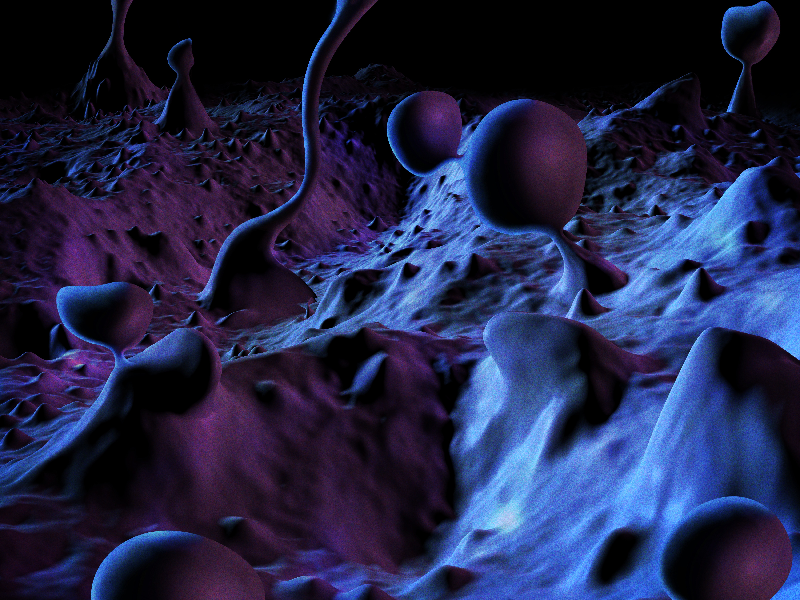
\includegraphics[width=1.\linewidth]{images/quantum_foam_2.png}
% 		\caption{An artists impression of the fluctuating nature of space-time at tiny distance scales, as expected in a quantum theory of gravity.}
% 		\vspace{-7pt}
% 		\label{fig:spacetime_foam}
% \end{wrapfigure}

% Einstein's theory of general relativity (GR) has been remarkably successful at describing the influence of gravity at macroscopic scales, but breaks down when applied to dense, compact systems such as black holes and the early Universe\todo{More about why GR and QM are incompatible}, and a quantum description of gravity must exist. Its effects however are typically expected to be strong at the \textit{Planck scale}, meaning colossal energies of $10^{19}$ GeV or minuscule distances of $10^{-35}$ m, and its effects are likely suppressed at the energy and distance scales we can experimentally probe and have thus far evaded detection.

% Although we do not have a complete quantum theory of gravity, we do know some of the features it is expected to exhibit. Most notably, the fabric of space-time itself would be subject to the intrinsic uncertainty present in all quantum theories and fluctuate at tiny distance scales~\cite{PhysRev.97.511, Hawking} (see Fig. \ref{fig:spacetime_foam}). The most straightforward consequence of this are so-called \textit{lightcone fluctuations}~\cite{PauliLightcone, Ford1999, gr-qc/9909085}, where the fluctuating space-time curvature causes variations in the time taken by a particle to travel between two points. Though these fluctuations would be very small, their effects could accumulate over large distances into measurable effects.

% It is also predicted that these space-time fluctuations manifest as so-called \textit{virtual black holes} (VBH)~\cite{Hawking1982,PhysRevD.53.3099}, microscopic black holes that form in the vacuum and promptly evaporate (the gravitational analogue of the virtual electron-positron pairs in the \textit{vacuum polarisation} phenomenon of electromagnetism). A neutrino encountering a VBH would undergo severe modifications to its propagation, with global symmetries potentially violated in the interaction~\cite{Anchordoqui:2005gj, PhysRevD.102.115003, Hellmann:2021jyz}, potentially resulting in flavour violations, conversions to different particle types or even the loss of the neutrino from the observable Universe altogether (REFs).

% % \textbf{State-of-the-art:} A broad range of experimental tests of quantum gravity and the structure of space-time have been performed, ranging from high precision photon interferometry laboratory experiments (REFs) to astrophysical observations of cosmic messenger particles such as $\gamma$-rays and gravitational waves from distant sources (REFs). There have also been experimental searches for the features predicted by some of the leading theories seeking to describe quantum gravity, such as the additional space-time dimensions predicted by string/brane theories (REFs), or violations of Lorentz invariance, $CPT$ symmetry or the weak equivalence principal (REFs). No signal of quantum gravity has been detected thus far however despite our knowledge that such a theory must exist, and without an accepted theory to guide us it is essential to perform the broadest range of tests possible and seek to continually increases sensitivity to these suppressed effects. \\

% % TODO neutrinos


% % It is also often predicted that these fluctuations can collapse to form so-called `virtual black holes' (VBH)~\cite{Hawking1982,PhysRevD.53.3099}, which are minuscule and quickly evaporate. Whilst this sounds exotic, it is in fact simply the gravitational analogue of the virtual electron-positron pairs that are fundamental to our understanding of the electromagnetic force. A neutrino encountering a VBH would likely experience significant disruption and/or loss of quantum information~\cite{hep-th/9508151}, resulting in decoherence. 



% % Neutrinos travelling from source to detector thus become increasingly out of phase with each other.

% % Though these fluctuations would be very small, their effects accumulate over large distances. It is also often predicted that these fluctuations can collapse to form so-called `virtual black holes' (VBH)~\cite{Hawking1982,PhysRevD.53.3099}, which are minuscule and quickly evaporate. Whilst this sounds exotic, it is in fact simply the gravitational analogue of the virtual electron-positron pairs that are fundamental to our understanding of the electromagnetic force. A neutrino encountering a VBH would likely experience significant disruption and/or loss of quantum information~\cite{hep-th/9508151}, resulting in decoherence. 

% % Particle's propagating in this fluctuating space-time 

% % In the absence of an accepted theory of quantum gravity, it is necessary to test many scenarios. A key feature expected in quantum gravity is that space-time itself is subject to the inherent uncertainty of quantum mechanics and fluctuates at very small distance scales~\cite{misner1973gravitation}. This is precisely the kind of stochastic environment that would produce neutrino decoherence~\cite{Mavromatos_2009,PhysRevD.102.115003}. %This project will exploit the unparalleled sensitivity of neutrinos to decoherence to search for both specific quantum gravity scenarios and a more general approach that is sensitive to decoherence effects from a broad range of sources. 

% % The most straightforward such decoherence mechanisms are so-called `lightcone' fluctuations\cite{Ford1999, gr-qc/9909085}, where the fluctuating space-time curvature causes the travel distance/time between two points to fluctuate. Neutrinos travelling from source to detector thus become increasingly out of phase with each other, leading to decoherence. Though these fluctuations would be very small, their effects accumulate over large distances. It is also often predicted that these fluctuations can collapse to form so-called `virtual black holes' (VBH)~\cite{Hawking1982,PhysRevD.53.3099}, which are minuscule and quickly evaporate. Whilst this sounds exotic, it is in fact simply the gravitational analogue of the virtual electron-positron pairs that are fundamental to our understanding of the electromagnetic force. A neutrino encountering a VBH would likely experience significant disruption and/or loss of quantum information~\cite{hep-th/9508151}, resulting in decoherence. 

% % % A stronger, highly promising signal occurs if these fluctuations sufficiently curve space-time sufficiently in a miniscule volume to collapse and form a singularity, creating a microscopic `virtual black hole' (VBH) which quickly evaporates (analogous to the well known virtual electron-positron pairs of the electromagnetic force). A neutrino encountering a VBH would likely experience significant wavefunction disruption and/or the loss of quantum information~\cite{hep-th/9508151}, which I have shown can produce observable effects even if only a small fraction of detected neutrinos experience such an event. 

% % % , which I have shown can produce observable effects even if only a small fraction of detected neutrinos experience such an event.

% % I have developed a phenomenological model of the influence of neutrino-VBH ($\nu$-VBH) interactions on neutrino propagation in a range of well motivated scenarios~\cite{PhysRevD.102.115003}, and remarkably have demonstrated that \textbf{sensitivity to Planck-scale physics can be achieved using the high-energy neutrinos detected by the IceCube neutrino observatory} (see Fig. \ref{fig:planck_scale_coherence_length}), even if only a small fraction of neutrinos undergo these encounters. I have recently also developed a model of neutrino decoherence from lightcone fluctuations\todo{Add referecnce once submitted} (submitted to PhysRevD), accounting for both fluctuating space-time curvature and also scenarios where the speed of light fluctuates for high energy particles  (so-called \textit{stochastic Lorentz invariance violation}~\cite{Vasileiou2015}). I will perform stringent experimental tests of these models in this project.

% \subsection{Neutrino oscillations and decoherence}

% \begin{wrapfigure}{R}{0.42\textwidth} %this figure will be at the right
%     \centering
% 		\vspace{-7pt}
% 		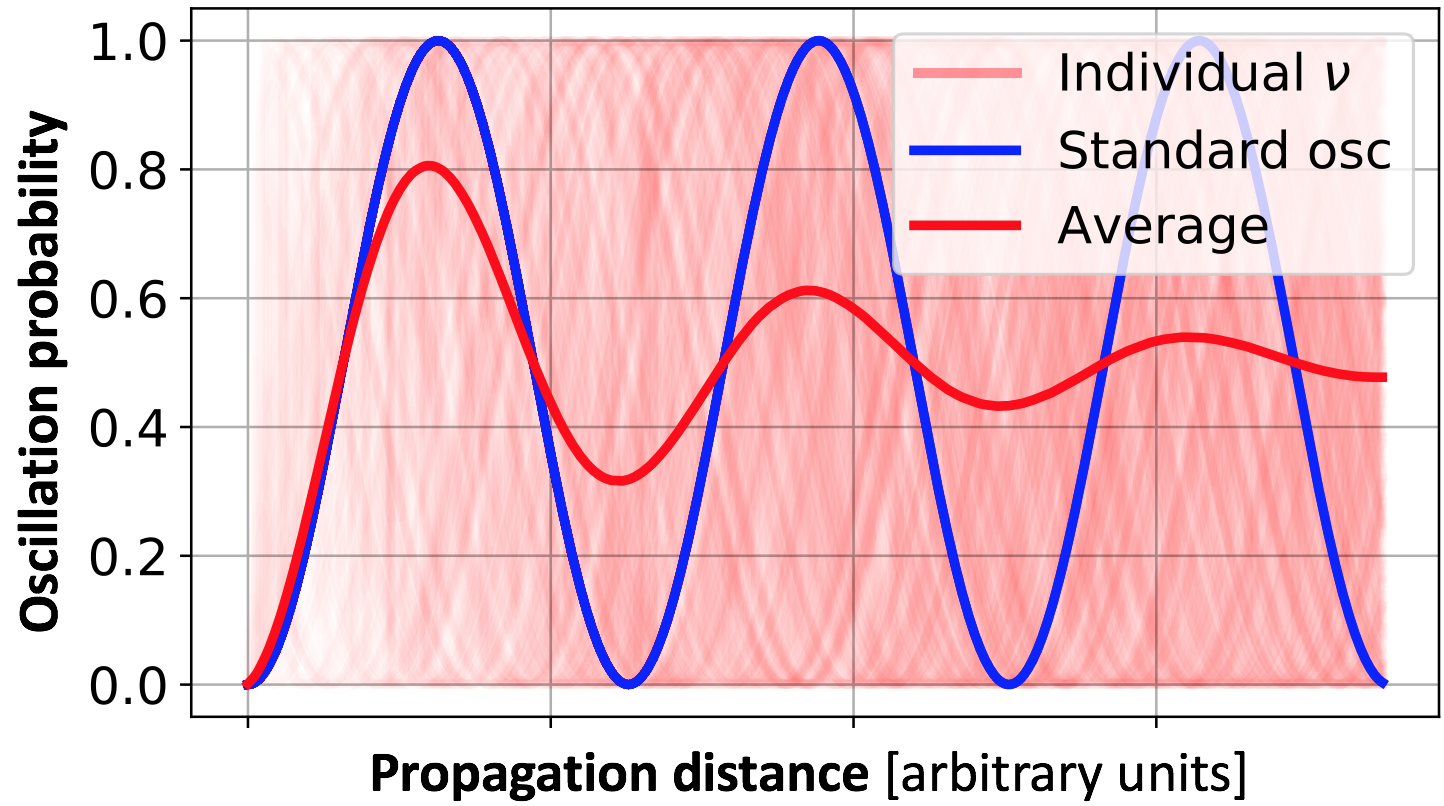
\includegraphics[width=1.\linewidth]{images/decoherence.png}
% 		\caption{Toy model example of individual neutrinos propagating in a fluctuating environment, which are perturbed and become increasingly out of phase, resulting in damping of the average oscillation probability.}
% 		\vspace{-5pt}
% 		\label{fig:decoherence}
% \end{wrapfigure}

% Neutrinos exhibit the peculiar phenomenon of \textit{neutrino oscillations} where a neutrino produced as one type (\textit{flavour}) may be detected later as another~\cite{Fukuda:1998mi, Ahmad:2001an,Ahmad:2002jz}. This is a consequence of mixing between neutrino mass and flavour states, and the detection of these oscillations implies that neutrinos have non-zero (albeit tiny) masses, contrary to the Standard Model (SM) of particle physics, providing one of the only confirmed experimental signs of Beyond Standard Model (BSM) physics today. These oscillations are characterised by \textit{mixing angles}, describing the mixing between mass/flavour states (controlling the oscillation amplitudes) and \textit{mass splittings}, which are the difference between the (squared) neutrino masses (controlling the oscillation frequencies), and the measurement of these oscillations is a major field of active research today.

% However, the quantum superposition effect producing these oscillations would be disrupted for neutrinos propagating in fluctuating space-time, resulting in the damping of neutrino oscillations and averaging of neutrino flavours in a process known as neutrino decoherence~\cite{Benatti_2000, PhysRevLett.85.1166}. The oscillating nature of neutrinos and their ability to travel vast distances unperturbed by the other forces of nature makes them uniquely sensitive to decoherence effects from quantum gravity, with the neutrinos acting as tiny quantum interferometers. Decoherence measurements are potentially sensitive to a range of new physics scenarios (REFs - grab from signal modelling section), including those only accessible via the gravitational force (to which nearly all other particle physics measurements are essentially blind)~\cite{Hellmann:2021jyz}.

% I have developed phenomenological models of the influence of neutrino-VBH ($\nu$-VBH) interactions on neutrino propagation in a range of scenarios (including flavor violations, democratic population of particle states, severe phase perturbations and total loss of the neutrino)~\cite{PhysRevD.102.115003}, and remarkably have demonstrated that the resulting damping effect from \textit{natural} Planck scale physics can be resolved using neutrino oscillation measurements by the IceCube neutrino observatory, even if only a small fraction of neutrinos undergo these encounters. I have also very recently developed a model of neutrino decoherence resulting from lightcone fluctuations~\cite{2103.15313} (submitted to the journal \textit{Phys. Rev. D}), accounting for both fluctuating space-time curvature and also scenarios where the speed of light is uncertain/variable for high energy particles (so-called \textit{stochastic Lorentz invariance violation}~\cite{Vasileiou2015}), yielding further potential signals in IceCube data. These models are the first to directly connect the potentially observable phenomenology of neutrino decoherence to the underlying microphysics of a quantum theory of gravity, allowing experimental constraints on the fundamental nature of space-time to be made using decoherence measurements for the first time in this project.

% \textbf{State-of-the-art:} Decoherence searches have been performed using neutrinos from nuclear reactors, the Sun, the Earth's atmosphere and particle accelerators, generally using simplified mathematical expressions rather than specific models, with no signal observed thus far. Despite the large distances travelled, neutrinos of extragalactic origin are not in general well suited to decoherence searches due to the incoherent nature of the sources of these neutrinos and degeneracies between the expected flavour composition in conventional vs. decoherence scenarios~\cite{PhysRevD.102.115003}. Decoherence effects resulting from quantum gravity are expected to be energy-suppressed, and the strongest constraints to these signals to date were set using low statistics publicly released IceCube data (by non-collaboration authors) (REF). The measurements I will perform will exceed the sensitivity of these results by orders of magnitude, measure new strongly energy-suppressed (cubic and quartic) scenarios that have not previously been experimentally tested, test an unprecedented range of specific models, and include a robust treatment of systematic uncertainties not present in previous works, representing a major leap forward in this exciting field. \\

% \todo{Proton decay}
% \todo{GRB lightcone}
% \todo{Lightcone holographic}

% % \noindent \textbf{State-of-the-art:} High er E and longer baseline at LBL.

% %I will perform stringent experimental tests of these models in this project.

% %Decoherence is highly suppressed and as yet unoberved for neutrinos

% % oscillations are coherent, meaning that the states of neutrinos of the same energy travelling the same path will evolve identically. This would be disrupted however if neutrinos couple to a stochastic environment in a process known as decoherence, observable as the \textbf{damping of neutrino oscillations} over distance (see Fig. \ref{fig:decoherence}). Decoherence is known in other quantum systems, but is highly suppressed and as yet unobserved for neutrinos due to their extremely feeble interactions with other (known) particles isolating them from their environment.

% % Neutrinos propagate as a superposition of three quantum states, giving rise to the peculiar phenomenon of \textit{neutrino oscillations} where a neutrino produced as one type (\textit{flavour}) may be detected later as another~\cite{Fukuda:1998mi, Ahmad:2001an,Ahmad:2002jz}. These oscillations are coherent, meaning that the states of neutrinos of the same energy travelling the same path will evolve identically. This would be disrupted however if neutrinos couple to a stochastic environment in a process known as decoherence, observable as the \textbf{damping of neutrino oscillations} over distance (see Fig. \ref{fig:decoherence}). Decoherence is known in other quantum systems, but is highly suppressed and as yet unobserved for neutrinos due to their extremely feeble interactions with other (known) particles isolating them from their environment.

% % I have developed a phenomenological model of the influence of neutrino-VBH ($\nu$-VBH) interactions on neutrino propagation in a range of well motivated scenarios~\cite{PhysRevD.102.115003}, and remarkably have demonstrated that \textbf{sensitivity to Planck-scale physics can be achieved using the high-energy neutrinos detected by the IceCube neutrino observatory} (see Fig. \ref{fig:planck_scale_coherence_length}), even if only a small fraction of neutrinos undergo these encounters. I have recently also developed a model of neutrino decoherence from lightcone fluctuations\todo{Add referecnce once submitted} (submitted to PhysRevD), accounting for both fluctuating space-time curvature and also scenarios where the speed of light fluctuates for high energy particles  (so-called \textit{stochastic Lorentz invariance violation}~\cite{Vasileiou2015}). I will perform stringent experimental tests of these models in this project.

% % Decoherence can result in a range of scenarios, including quantum gravity, neutrino interactions with Dark Matter~\cite{1909.11271, EPJC802020}, string theory~\cite{Ellis:1997jw,doi:10.1142/S0217732397000248,PhysRevD.80.124019,Mavromatos2010}, diffuse gravitational waves~\cite{Dvornikov_2020}, and can reveal whether neutrinos are their own antiparticle~\cite{CAPOLUPO2019298, 2001.07580}. Decoherence measurements can thus confront some of the biggest questions in particle physics.


% \subsection{$CPT$ violation and matter-antimatter asymmetry}

% \textbf{TODO Need a new $CPT$-V figure, choose a less extreme scenario rather than trying to motivate the full E range (decoherence does that already)}

% % % \begin{wrapfigure}{R}{0.43\textwidth} %this figure will be at the right
% % \begin{wrapfigure}{R}{0.43\textwidth} %this figure will be at the right
% %     \centering
% %     % \vspace{-9pt}
% %     \includegraphics[trim=0.0cm 0.0cm 0.cm 0.0cm, clip=true, width=1.\linewidth]{images/CPTv_IceCube.pdf}
% % 	\caption{Difference between neutrino and antineutrino oscillation probability in the presence of $CPT$-V, showing potential signals that no experiment other than IceCube could detect. No difference is expected if $CPT$ is not violated, meaning any observed difference must result from new physics. }
% % % 	\vspace{-7pt}
% % 	\label{fig:$CPT$v}
% % \end{wrapfigure}

% Like other particles, neutrinos have antimatter counterparts known as antineutrinos, which have mirrored but otherwise identical properties. However, if gravity is a quantum force then the uncertain nature of space-time \todo{More specific here} can result in differing properties between matter and antimatter, known as \textbf{$CPT$ violation} ($CPT$-V)~\cite{Mavromatos:2005mi, AmelinoCamelia:2008qg, RalfLehnert:2016grl}. For example, $CPT$ symmetry is only valid in (a) flat space-time, and thus may be violated due to the fluctuating microscopic nature of  space-time in a quantum theory of gravity, and (b) a \textit{unitarity} quantum theory (one where quantum information/probability is conserved), whereas in a Universe permeated by VBHs quantum information could be lost beyond these microscopic event horizons, resulting in apparent violations of unitarity and $CPT$ symmetry~\cite{Mavromatos:2005mi}. More generally, $CPT$-V is a frequent prediction of the many variations and developments of potential quantum gravity theories such as string theory~\cite{Mavromatos:2005mi, Hashimoto:2014aoa, Ellis:2013gca}.

% For neutrinos, $CPT$-V predicts \textbf{differing oscillation frequencies and amplitudes between neutrinos and antineutrinos} through differing mass splittings and mixing angles~\cite{Barenboim:2017ewj}, a potentially observable signal. These effects are likely suppressed at energies below the Planck scale, but this can be partially overcome in the high energy measurements of neutrino oscillations with IceCube (orders of magnitude higher in energy than any other experiment) to yield \textbf{sensitivity to signals to which all other experiments would be blind} (see Fig. \ref{fig:$CPT$v}). 

% Detecting $CPT$-V would have profound consequences even beyond the search for quantum gravity. One of the biggest questions in physics is why the Universe appears to almost entirely consist of matter, and not antimatter, since (in the absence of $CPT$-V or other new physics) both are expected to have been produced equally~\cite{Sakharov_1991}. The very fact we are even here to ponder this question is a consequence of this, since without this imbalance all matter and antimatter would have annihilated to leave a Universe devoid of stars, planets or life. Known differences between matter/antimatter (so-called $CP$-violations) can only account for a tiny fraction of the observed imbalance, meaning that \textbf{new physics like $CPT$-V must exist}. The energy-suppressed $CPT$-V I will search for is an excellent candidate to explain this, as these effects would have been strong in the high temperatures of the early Universe when (anti)matter was forming~\cite{Mavromatos:2017cxr, hep-ph/9809542, Ellis:2013gca}. Furthermore, tensions have emerged in neutrino vs antineutrino oscillation measurements~\cite{Abe:2019vii,NOvA_CP_result}, potentially indicating the presence of new physics that this project could reveal, making this measurement more important than ever.

% % \todo{More generally $CPT$-V from scattering on matter/backgrounds~\cite{Capolupo:2020myw}? Maybe motivate with the fact that standad matter effects are $CPT$ violating, and so $CPT$ effects from unknown backgrounds are well motivated.}

% \noindent \textbf{State-of-the-art:} In the absence of a concrete model of quantum gravity (or other $CPT$-V theory) it is essential to probe the broadest possible range signals~\cite{hep-ph/9809542} for signs of $CPT$-V. Experimental constraints exist for neutral kaons (REFs), neutrinos~\cite{Adamson:2013whj, Ohlsson:2014cha}, hadron colliders~\cite{vanTilburg:2016awx} and in precision tests of low energy systems such as particle magnetic moment measurements (REFs) and (anti)hydrogen spectroscopy~\cite{Kostelecky:2015nma}, with no observed signal to date. This indicates that such effects must be highly suppressed, as expected in a quantum theory of gravity. The sensitivity of neutrino oscillations to very small (sub-eV) mass differences makes them one of the best motivated search channels~\cite{PhysRevD.99.075022}, and the measurements in this work will test $CPT$-V at orders of magnitude higher energies that existing limits with accelerator neutrinos. Additionally, under my leadership the precision of IceCube's neutrino oscillation measurements has reached parity with accelerator experiments for the first time, and will surpass this during this project with the data from the next-generation IceCube Upgrade. Coupled with pioneering (anti)neutrino separation methods I will develop, this project will afford unparalleled sensitivity to energy-suppressed $CPT$-V in neutrino oscillations\todo{Mention strongest constrains for osc specifically}. \\


% % The concept of \textit{symmetries} in physics are fundamental to understanding of the microscopic world. 
% % Charge-Parity-Time ($CPT$) symmetry - meaning that the physics of a system remains unchanged when simultaneously the charge flips, directions are mirrored and the direction of time reverses - is a cornerstone of the quantum field theories that have described our Universe at microscopic scales with unprecedented success. However, the fundamental conditions required for $CPT$ symmetry are not expected to hold in a quantum theory of gravity (for example due to the fluctuating nature of space-time), leading to the prediction that $CPT$ symmetry may be violated at some energy scale~\cite{Mavromatos:2005mi, RalfLehnert:2016grl}. An experimental signature of $CPT$ violation ($CPT$-V) would be a game changing result in the search for quantum gravity and more generally would shake the foundations of quantum field theories.

% % A potential consequence of $CPT$-V is differing properties such as mass between particles and antiparticles, which for neutrinos would manifest as differing oscillations for neutrinos and antineutrinos~\cite{Ohlsson:2014cha, Barenboim:2017ewj}. Such effects have been probed with neutral kaons and neutrinos~\cite{TAKEUCHI201279, Adamson:2013whj}, but I have identified that the atmospheric neutrino oscillations observed by IceCube (orders of magnitude higher energy than any other experiment) are likely far more sensitive to such effects, given that $CPT$-V (and other effects of Planck scale physics) are expected to be suppressed at low energies. Fig. \ref{fig:$CPT$v} shows two example $CPT$-V scenarios (in an energy-dependent model I have developed) that produce significant effects for IceCube but would not have been detected by previous searches with accelerators, and I will perform the world's most sensitive search for energy-dependent $CPT$-V. 


% % \todo{Another possible manifestation...}Additionally, potential $CPT$-V effects in neutrino decoherence have been identified~\cite{Mavromatos_2009, Barenboim:2004wu, Carrasco:2018sca}, providing a powerful synergy between the elements of this proposal. I have shown that such effects can produce potentially observable signals for high energy neutrinos in IceCube, and will also test these effects in this work. 


% \subsection{The IceCube neutrino observatory and the IceCube Upgrade}

% % \begin{wrapfigure}{R}{0.5\textwidth} %this figure will be at the right
% %     \centering
% % 	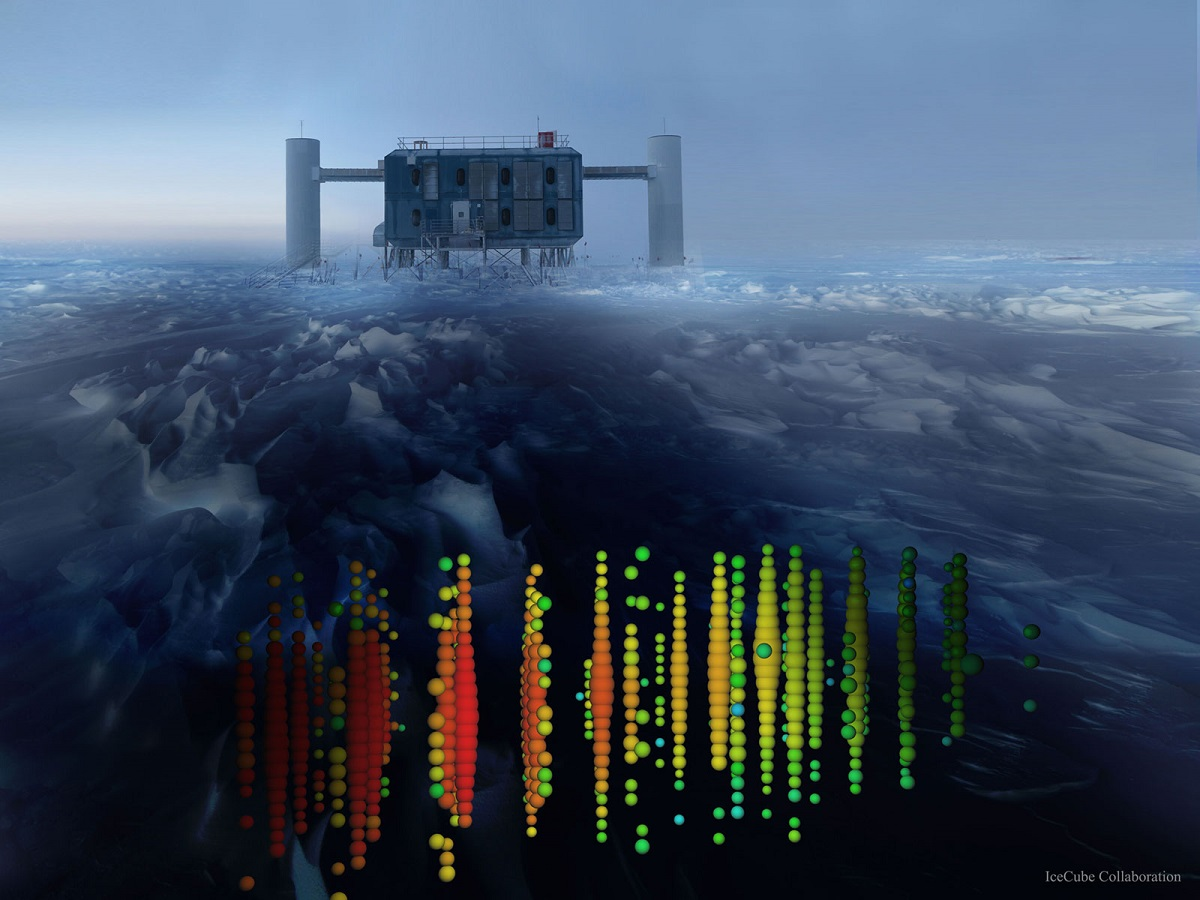
\includegraphics[width=1.\linewidth]{images/IceCube_1200x.jpg}
% % 	\caption{The IceCube neutrino observatory at the South Pole. Cherekov light from neutrino interactions in the glacial ice deep below the surface are detected by PMTs.}
% % % 		\vspace{-7pt}
% % 	\label{fig:atmo_osc}
% % \end{wrapfigure}

% % \begin{figure}
% % %\begin{subfigure}[t]{0.5\textwidth}
% %     \begin{subfigure}[c]{0.65\textwidth}
% %     \centering
% %     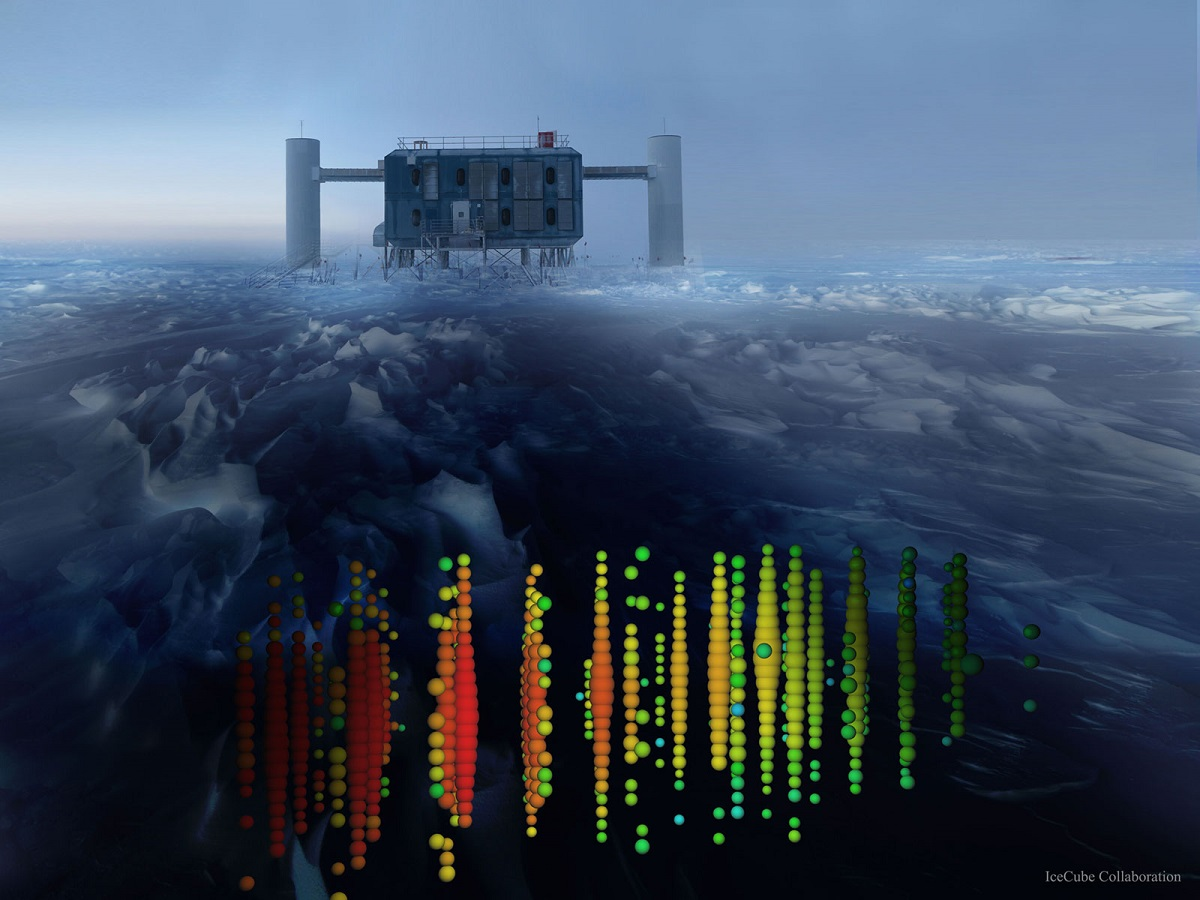
\includegraphics[width=0.9\linewidth]{images/IceCube_1200x.jpg}
% %     \caption{\label{fig:icecube}}
% %     \end{subfigure}
% %     \begin{subfigure}[c]{0.35\textwidth}
% %     \centering
% %     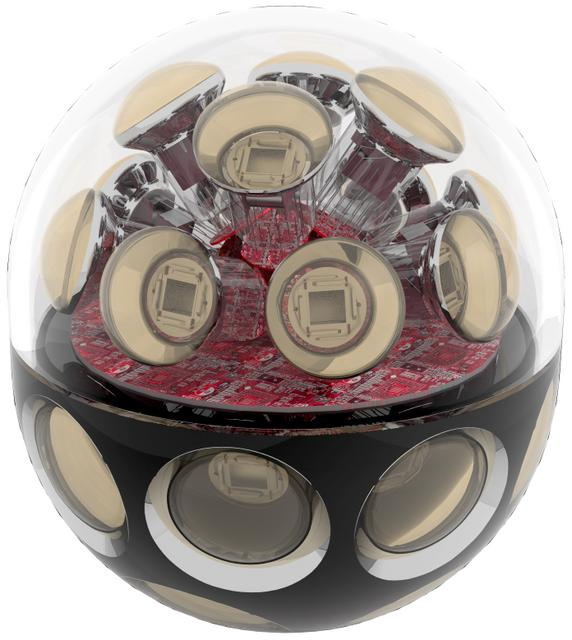
\includegraphics[width=0.9\linewidth]{images/mdom.jpg}
% %     \caption{\label{fig:mDOM}}
% %     \end{subfigure}
% %     \caption{(a) The IceCube neutrino observatory at the South Pole. Cherekov light from neutrino interactions in the glacial ice deep below the surface is detected by PMTs. (b) One of the new multi-PMT optical modules to be installed in the IceCube Upgrade.}
% % \end{figure}

% The IceCube neutrino observatory~\cite{Aartsen_2017}, located at the geographic South Pole, instruments a vast 1 billion tons of glacial ice deep below the surface with 5160 optical sensors, each containing a single photomultipier tube (PMT), to detect Cherenkov light produced by the interactions of neutrinos in the ice. This truly colossal 1 Gton detector detects huge numbers of neutrinos produced in air showers when cosmic rays slam into the Earth's atmosphere, many of which oscillate from muon to tau flavoured as they cross the Earth (Fig. \ref{fig:atmo_osc}), as well as neutrinos of extra-galactic origin. These neutrinos are detected across a staggering six orders of magnitude in energy (GeV to PeV), dwarfing the energy reach of even particle colliders. 

% %These high-energy neutrinos with long travel distances are perfect to search for decoherence from Planck-scale physics, and the huge statistics allows even very weak effects to be probed (crucial for quantum gravity). 

% % \begin{wrapfigure}{R}{0.4\textwidth} %this figure will be at the right
% %     \centering
% % 	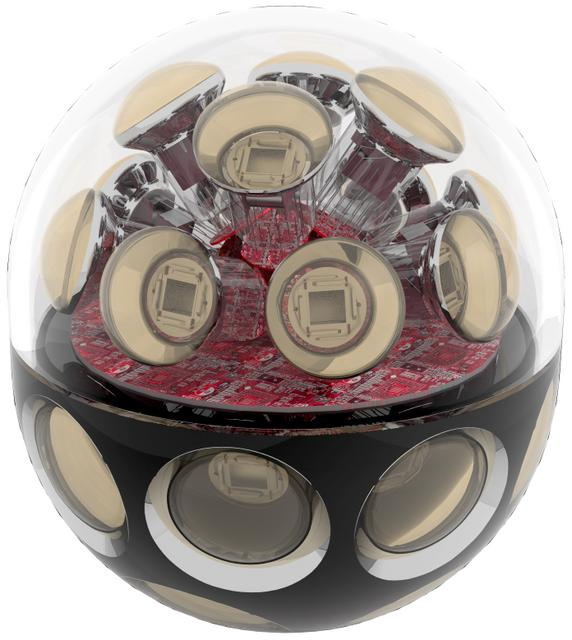
\includegraphics[width=1.\linewidth]{images/mdom.jpg}
% % 	\caption{One of the new multi-PM optical modules to be installed in the IceCube Upgrade.}
% % % 		\vspace{-7pt}
% % 	\label{fig:mDOM}
% % \end{wrapfigure}


% Furthermore, in 2023-24 IceCube will be substantially upgraded~\cite{IceCubeUpgrade_ICRC2019} with sensitive new multi-PMT optical modules, dramatically increasing the instrumentation density in a 2 Mton core. I lead the international group conducting the simulation studies of the goals and performance of the IceCube Upgrade experiment~\cite{IceCubeUpgrade_ICRC2019, NuFactProceedings}, which show factor 2-4 improvements in detector efficiency and resolution, providing a truly next-generation precision neutrino physics facility. Additionally, a host of new calibration devices will be deployed to allow precise characterisation of the natural detection medium and significantly reduce systematic uncertainties.\\



% ------------------------------------------------------------------------------
% ------------------------------------------------------------------------------
% ------------------------------------------------------------------------------
% ------------------------------------------------------------------------------

\subsection{Methodology}
\vspace{0.1 cm}

% \textbf{From instructions:} Describe the proposed methodology in detail including any key
% intermediate goals. Explain and justify the methodology in relation to the state of the art, and
% particularly novel or unconventional aspects addressing the 'high-risk/high-gain' balance. Highlight
% any intermediate stages where results may require adjustments to the project planning. 

\todo{Do I need more info on IceCube in here?}


The core deliverables of this project are the world's most sensitive (and in many cases first) searches for unique signatures of quantum gravity and the underlying nature of space-time, and for deviations between the properties of neutrinos and antineutrinos. In doing so and my team (one postdoc, two PhD students) and I are attempting to discover the first underlying indication of a unifying model of gravity at subatomic scales and an explanation for the overwhelming pervasiveness of matter rather than antimatter in the Universe. \\


\subsubsection{Neutrino-antineutrino separation}

\begin{figure}
%\begin{subfigure}[t]{0.5\textwidth}
    \begin{subfigure}[b]{0.5\textwidth}
    \centering
    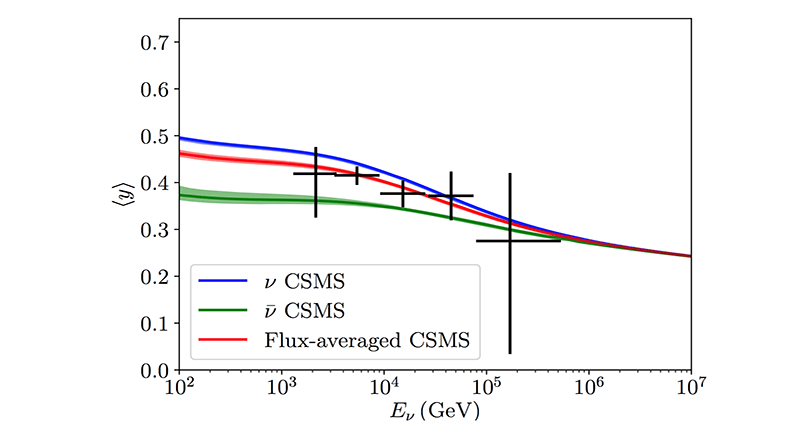
\includegraphics[trim=2.0cm 0.0cm 1.0cm 0.0cm, clip=true, width=\linewidth]{images/inelasticity.png}
    \caption{\label{fig:inelasticity}}
    \end{subfigure}
    \begin{subfigure}[b]{0.5\textwidth}
    \centering
    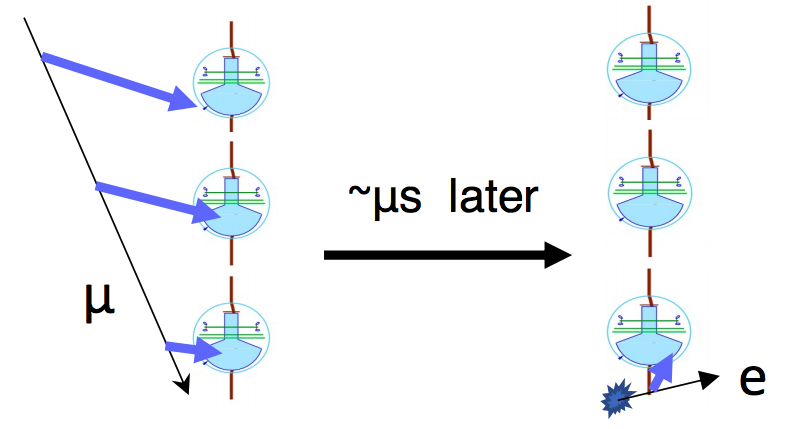
\includegraphics[trim=0.0cm 0.0cm 0.0cm 0.0cm, clip=true, width=\linewidth]{images/michel_electron.png}
    \caption{\label{fig:michel_electron}}
    \end{subfigure}
    \caption{(a) The average inelasticity, $\langle y \rangle$, of neutrino (blue) and antineutrino (green) interactions in IceCube, which differs in the energy range probed in this work~\cite{Aartsen:2018vez}. Reconstructing the inelasticity in IceCube events can thus be used to distinguish (anti)neutrino interactions. (b) A muon ($\mu$) from a neutrino interaction deposits light in the detector (leading to a reconstructable track) before stopping. Microseconds later the stopped muon decays, producing a Michel electron ($e$) which itself produces detectable light in the nearest sensor.}
\end{figure}

The most challenging but highest impact technical aspect of this project is the development of the first neutrino-antineutrino discrimination techniques to be used in neutrino oscillation measurements in IceCube, enabling the pioneering $CPT$-V measurements I will make. The properties of the neutrino interactions observed by IceCube that can separate these are;

\begin{itemize}
    \item The \textit{inelasticity} of the event, meaning the fraction of the incoming neutrino energy transferred to the ice nucleus in the interaction, which is on average $\sim$10-50\%  higher for neutrinos than antineutrinos in the energy range of interest (see Fig. \ref{fig:inelasticity}).
    \item The (anti)muons produced in muon (anti)neutrino interactions eventually come to rest and decay in the ice, producing a \textit{Michel electron} that yields delayed light a few microseconds later in the detector ($\sim$5000 photons per decay). The lifetime of this decay differs for muons and antimuons due to capture of muons on oxygen nuclei in the ice, meaning that the time of this delayed light can distinguish between neutrino and antineutrino events (see Fig. \ref{fig:michel_electron}). 
\end{itemize}

The reconstruction of muon neutrino inelasticity in IceCube was first achieved for TeV neutrinos~\cite{Aartsen:2018vez}, and recently I have demonstrated that inelasticity reconstruction with $\sim$30\% precision precision is possible even for for lower energy GeV events where neutrino oscillation signals are strong, and with the more densely instrumented IceCube Upgrade a precision of $\sim$10\% is expected. Additionally, the IceCube oscillation physics working group I lead has recently demonstrated the feasibility of detecting the delayed light from Michel electrons (observing such light in $\sim$5\% of events). The new sensors of the IceCube Upgrade will be far more sensitive to this dim delayed light signal, and the much improved track reconstruction capabilities will allow the location of the muon decay (and thus the expected location of the delayed light signal) to be precisely determined.

I will build on these initial studies to pioneer the first use (anti)neutrino separation in IceCube neutrino oscillation measurements, using machine learning classification methods to combine both reconstructed inelasticity and delayed light detection (alongside correlating data features) to predict whether an even is a neutrino or antineutrino and achieve statistically separated data samples. To do so I will build upon my existing machine learning collaborations with experts from the ATLAS collaboration at the LHC, and exploit the vast flux of muons from cosmic ray air showers observed by IceCube to perform high statistics tests of delayed light tagging methods independently of the neutrino signals.

\textbf{Risk/Gain:} This a central and highly challenging element of this project, requiring the development and integration of multiple brand new experimental methods. However, a successful (anti)neutrino classifier will be truly game-changing for IceCube oscillation physics, paving the way for new physics searches with differing (anti)neutrino signals including Non-Standard Interactions (likely yielding the first constraints on the imaginary components of such effects for some couplings), sterile neutrinos and the determination of the neutrino mass ordering, not to mention the $CPT$-V searches in this project. These methods can also be used to probe the antineutrino content of the astrophysical neutrino flux observed by IceCube (REF), constraining their production mechanisms (a major open question in neutrino astronomy) (REF Glashow paper). I will publish a dedicated paper on these pioneering methods in a suitable technical journal, such as the \textit{Journal of Instrumentation}. \\


\subsubsection{Simulations}

\begin{wrapfigure}{R}{0.35\textwidth} %this figure will be at the right
    \centering
    % \vspace{-7pt}
    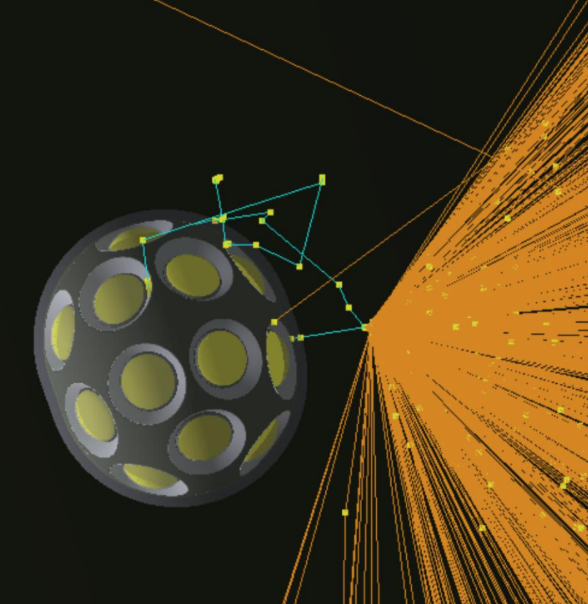
\includegraphics[trim=0.0cm 0.0cm 0.cm 1.0cm, clip=true, width=\linewidth]{images/mDOM_noise.png}
    % \end{subfigure}
    \caption{Visualisation of a prototype GEANT4 simulation of one of the new optical sensors in the IceCube Upgrade. A radioactive decay event is shown.}
    % \vspace{-7pt}
    \label{fig:mDOM_sim}
\end{wrapfigure}

The fundamental method used in these measurements is the comparison of simulated new physics signals and resulting detector response to observed data. I will develop software models of the geometry, active photo-multiplication stage (including spurious pre/after-pulsing) and readout electronics for the new optical modules in the IceCube Upgrade, for the first time utilising the `industry standard' \texttt{GEANT4}(REF) software package to replace the simple and imprecise parameterisations currently used in IceCube simulations. A particular challenge will be modelling the correlated noise across the segmented optical modules resulting from the decays of trace radioactive impurities in the glass pressure spheres surrounding the sensors, and calibrating this for every individual sensor. I will verify and tune these models against laboratory test data from my collaborators in Germany and the US and ultimately using the first data from the deployed detector, with my team travelling to the South Pole to assist the detector installation and utilise these simulations to verify the operation of the deployed hardware in real-time. It is therefore crucial that these simulations are complete at the time the detector installation commences, and so this work is prioritised at the start of the project, and indeed this project is critical to the success of the IceCube Upgrade physics program and will be used in all future measurements by this 300-person international collaboration. I will publish a methods paper describing these models and the methods employed in a suitable technical journal (e.g. the \textit{Journal of Instrumentation}). \\

I will then use these detector modelsin combination with state-of-the-art event generator software to produce high statistics Monte Carlo (MC) simulation samples of both neutrino interactions and background events (atmospheric muons and coincident detector noise) in the detector for comparison to observed data in these measurements. Recent developments in the \texttt{GENIE} (REF - High E version) neutrino event generator software will be utilised to enable consistent modelling of neutrino interactions across the vast energy span encompassed by these measurements for the first time, and I will also integrate cross section tuning data provided by accelerator neutrino experiments. 

Under my leadership as \textit{IceCube Upgrade simulation manager}, my collaborators and I have developed initial prototypes of these simulations (see Fig. \ref{fig:mDOM_sim}), which were fundamental to demonstrating the physics potential of the IceCube Upgrade and its successful funding. This, combined with my experience in high fidelity detector modelling from my Ph.D. -- where I developed simulations of the tracking tracking detector the Fermilab muon g-2 experiment, which were a fundamental component of the most precise high energy particle physics measurement in history (REF) -- and four years of experience as a professional simulations engineer in the space industry before my academic career (developing simulations of the European Space Agency's ExoMars Rover, Solar Orbiter and GAIA missions), makes me ideally suited to this task. \\



\subsubsection{Event sample}

At the core of these measurements will be the first \textbf{atmospheric neutrino data sample spanning the full energy reach of IceCube} (GeV to PeV), containing well over \textbf{1 million neutrinos} to provide unprecedented statistics for neutrino physics. The core challenges for this sample are to reject $\mathcal{O}(10^6)$ atmospheric muon and coincident noise background events for every neutrino to produce a pure neutrino sample, and to reconstruct the properties of these neutrino interactions (for example the energy, direction and flavour). 

To this end I will unify the disparate existing methods developed by myself (GeV energies) and my collaborators (TeV energies) and extend them to exploit the new sensor data from the IceCube Upgrade, and the sample must support event characteristics ranging from $\mathcal{O}$(m) scale 1 GeV events lighting up just a few optical modules to 100s of TeV muon tracks (from uncontained muon neutrino charged current interactions) travelling multiple km through the ice.  The noise rates will be orders of magnitude higher in the IceCube Upgrade than the existing IceCube array, but I will supress this by exploiting the segmented and densely packed nature of the new sensors to veto detector triggers with light signatures causally inconsistent with a common source, building upon my experience developing the most powerful noise rejection methods in IceCube to date.

\textbf{Risk/Gain:} Fully exploiting the new optical modules requires developments of entirely new neutrino reconstruction techniques, and the development of deep learning neural network reconstructions methods that are not tied to the regular pixel structure assumed standard image processing techniques (which dominate much of the machine learning community) is well underway within the IceCube collaboration. In fact, a graph neutral network (GNN) based method resulting from my collaboration with machine learning experts from the ATLAS experiment has already demonstrated $\sim$30\% improvement in resolution over the current state-of-the-art methods. Bringing these methods to maturity and for the full range of event topologies encountered in this sample will be a major challenge for my group and our collaborators, but will yield major leaps in resolution and thus measurement precision \todo{mention fall back}. \\



\subsubsection{Systematic uncertainties}

The large statistical power of these measurements and weakness of the sought-after signals demand a robust treatment of systematic uncertainties. Utilising the experience from simulation development, I will perform simulation studies of the impact of detector calibration uncertainties on the analyses, including the PMT quantum efficiency, noise rates and position/orientation of the new optical sensors -- which are deployed down 2 km long cables into melted and subsequently re-frozen boreholes in the ice -- and the optical properties of these re-frozen ice columns. These uncertainties will also be reduced using the new calibration devices deployed with the IceCube Upgrade.

The composition of the atmospheric neutrino flux is a major source of systematic uncertainty due to uncertainties in the spectrum of cosmic rays reaching the Earth, atmospheric conditions, and the modelling of hadronic processes governing the air shower development. I will exploit the copious flux of atmospheric muons detected by IceCube ($\mathcal{O}(10^5)$ per neutrino) to develop a high statistics `sideband' sample of well reconstructed muons and simultaneously fit this data sideband alongside the neutrino data during these measurements, both strongly constraining the air shower uncertainties and acting as a control sample for evaluating the modelling of the detector independently of the neutrino physics signals, and thus increasing both the sensitivity and robustness of these measurements. This will be the first use of this novel method in IceCube. \\

%There is synergy here with ongoing activities at NBI, where a muon sample is being developed for calibration of the quantum efficiency of the PMTs which can serve as a starting point for this sideband to accelerate its development.  \\


\subsubsection{Signal modelling}

I will model the influence of the new physics probed in this work on neutrino propagation using the state-of-the-art \texttt{nuSQuIDS} quantum state evolution software~\cite{Delgado:2014kpa, nusquidsGIT}, building on my experiences implementing my $\nu$-VBH interaction model~\cite{PhysRevD.102.115003}, and including an accurate treatment of the interplay between these signals and standard matter in the Earth on neutrino propagation (including absorption of high energy neutrinos by the Earth), which has been neglected in many earlier decoherence studies (in some cases leading to spurious signal artefacts)~\cite{PhysRevD.97.115017}. 

Both decoherence and $CPT$-V have been predicted from varied new physics scenarios, meaning these measurements are potentially sensitive to the properties of string theories~\cite{Mavromatos2010, AmelinoCamelia:2008qg}, black hole information theory (REFs), new particles~\cite{Hellmann:2021jyz}, neutrino interactions with Dark Matter~\cite{1909.11271, EPJC802020, Capozzi:2018bps, 1904.02518} and the diffuse gravitational wave background~\cite{PhysRevD.100.096014}. To this end I will host a specialised workshop on neutrino decoherence and $CPT$-V to further develop these scenarios (drawing upon the \textit{COST Action CA18108 (quantum gravity phenomenology)} network of which I am an active member) with a view to testing further models in this project, and expect to create a number of MSc projects developing this phenomenology, potentially yielding dedicated publications. \\


\subsubsection{$CPT$-V and decoherence data analysis}

\begin{figure}
%\begin{subfigure}[t]{0.5\textwidth}
    \begin{subfigure}[b]{0.5\textwidth}
    \centering
    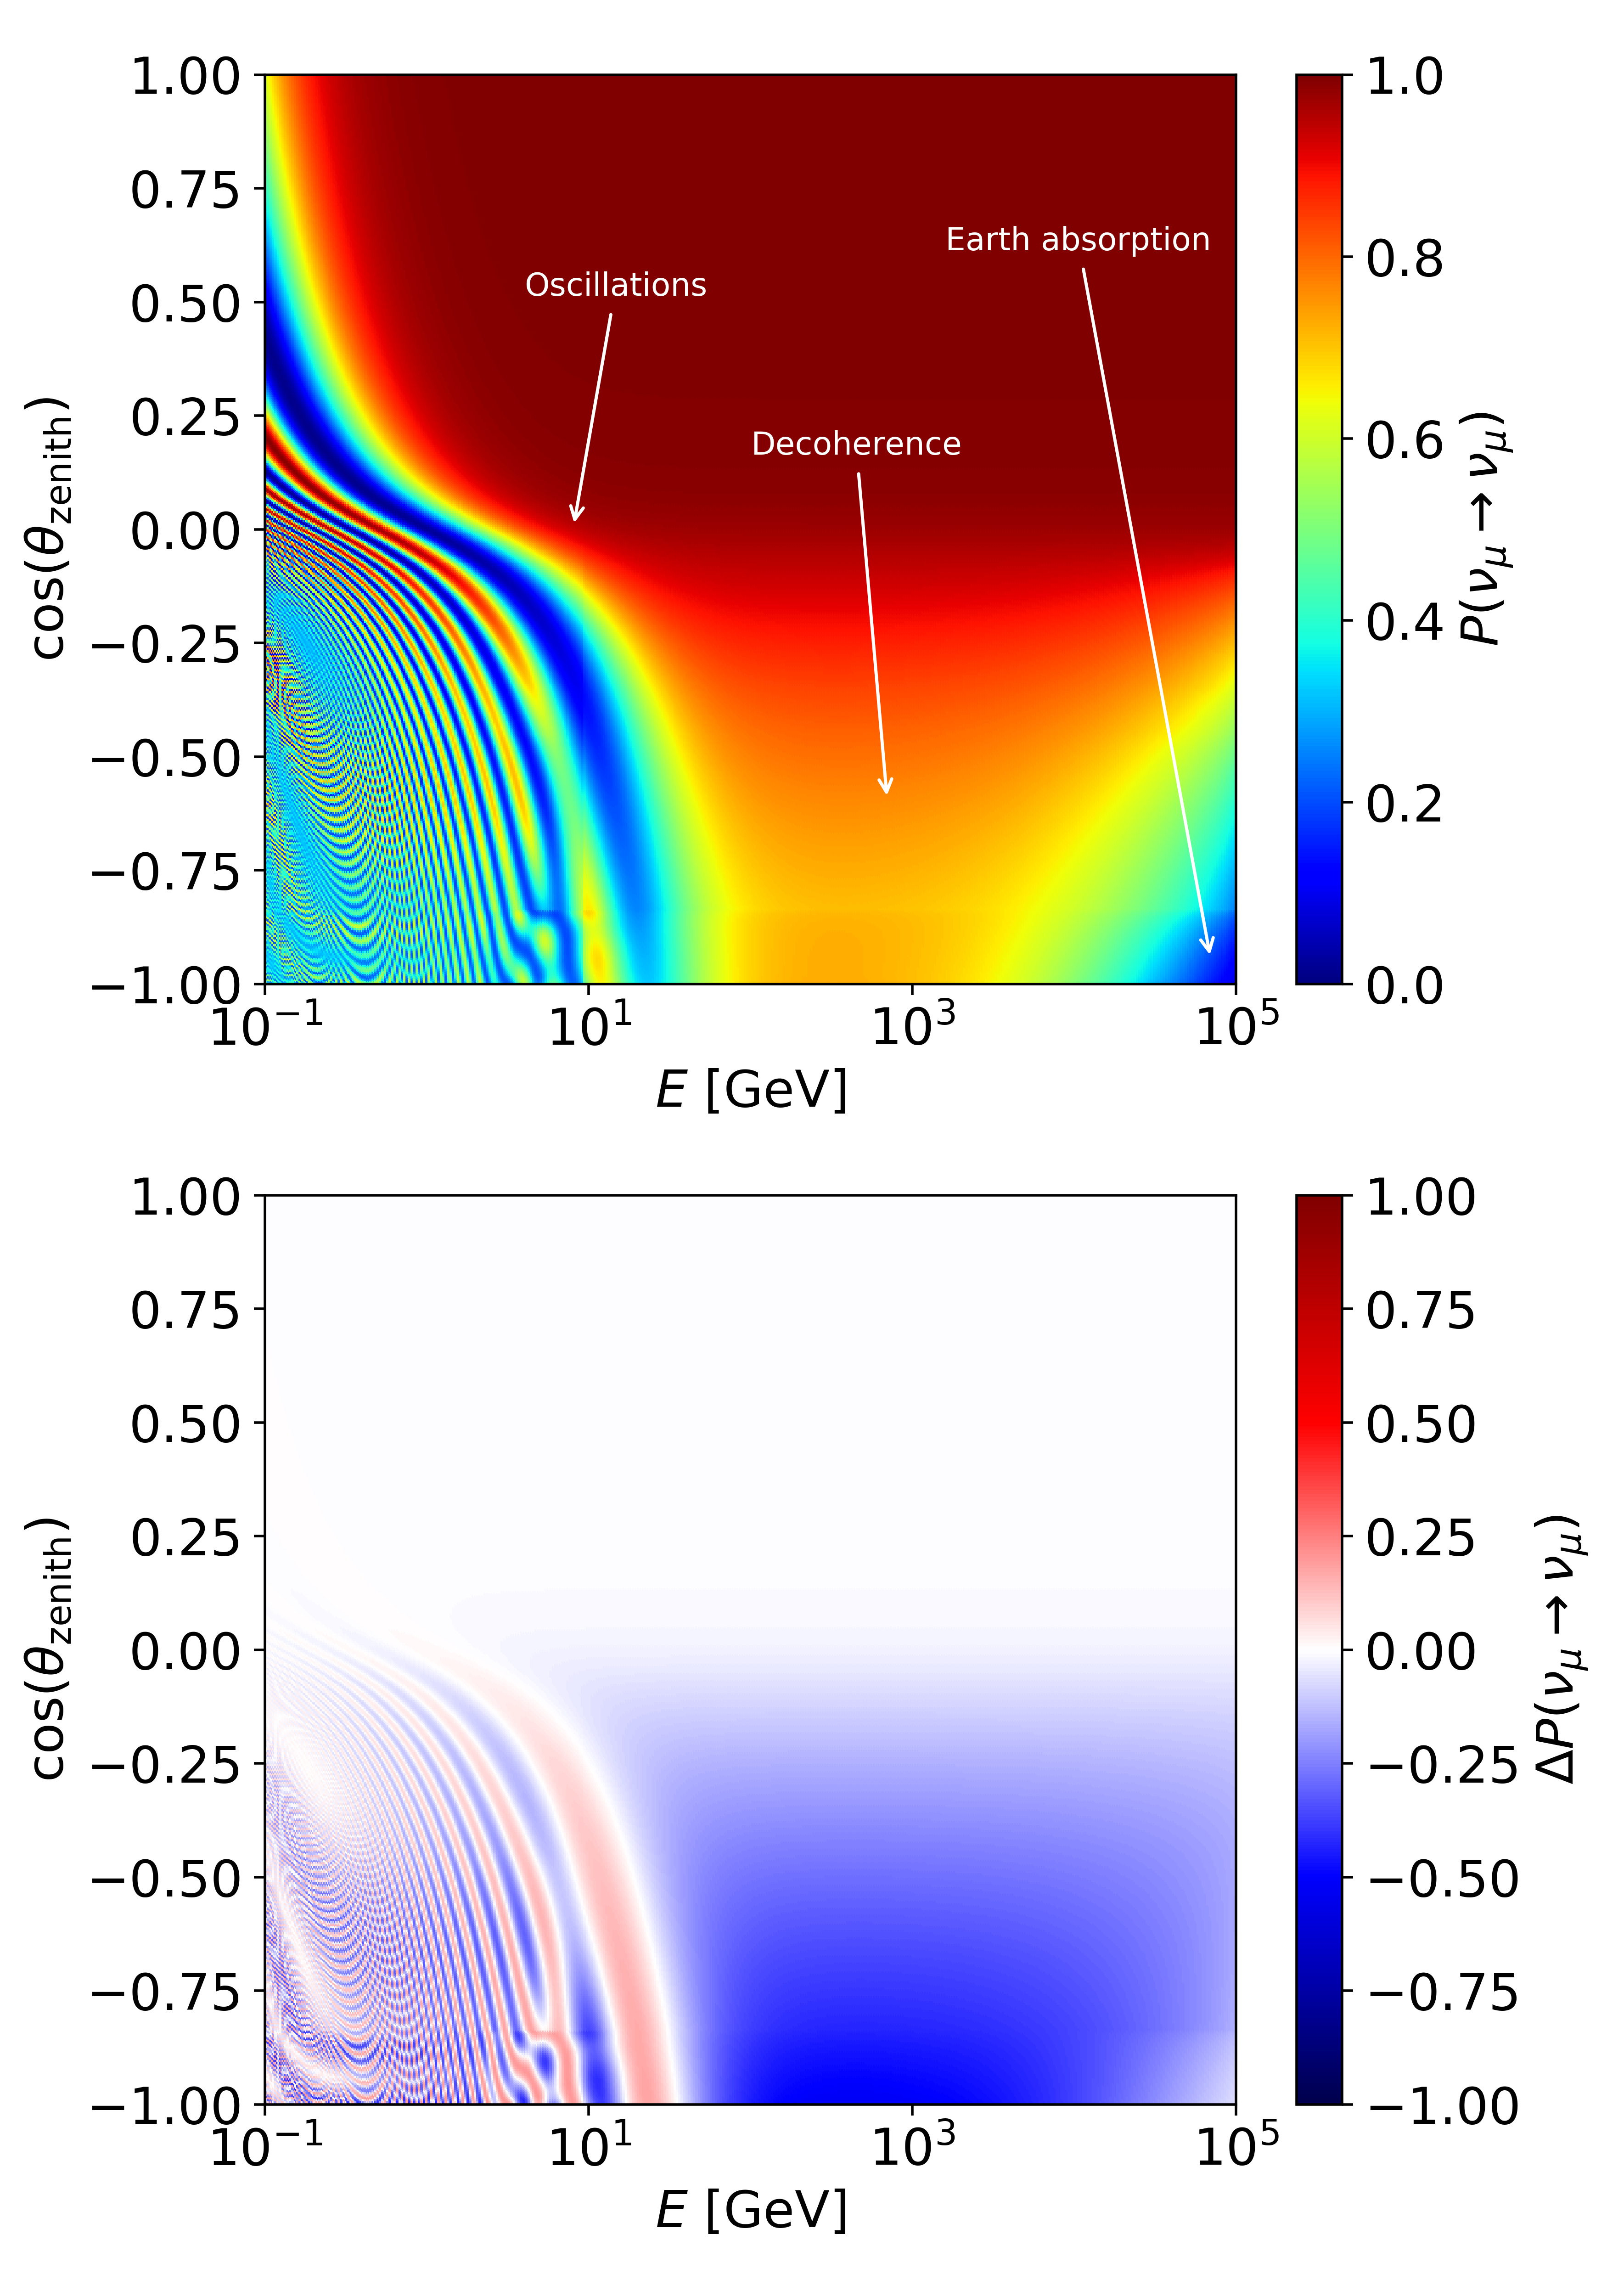
\includegraphics[trim=0.0cm 12.7cm 0.cm 0.2cm, clip=true, width=1.\linewidth]{images/atmo_oscillogram_randomize_flavor_n0_matter.png}
    \caption{}
    \end{subfigure}
    \begin{subfigure}[b]{0.5\textwidth}
    \centering
    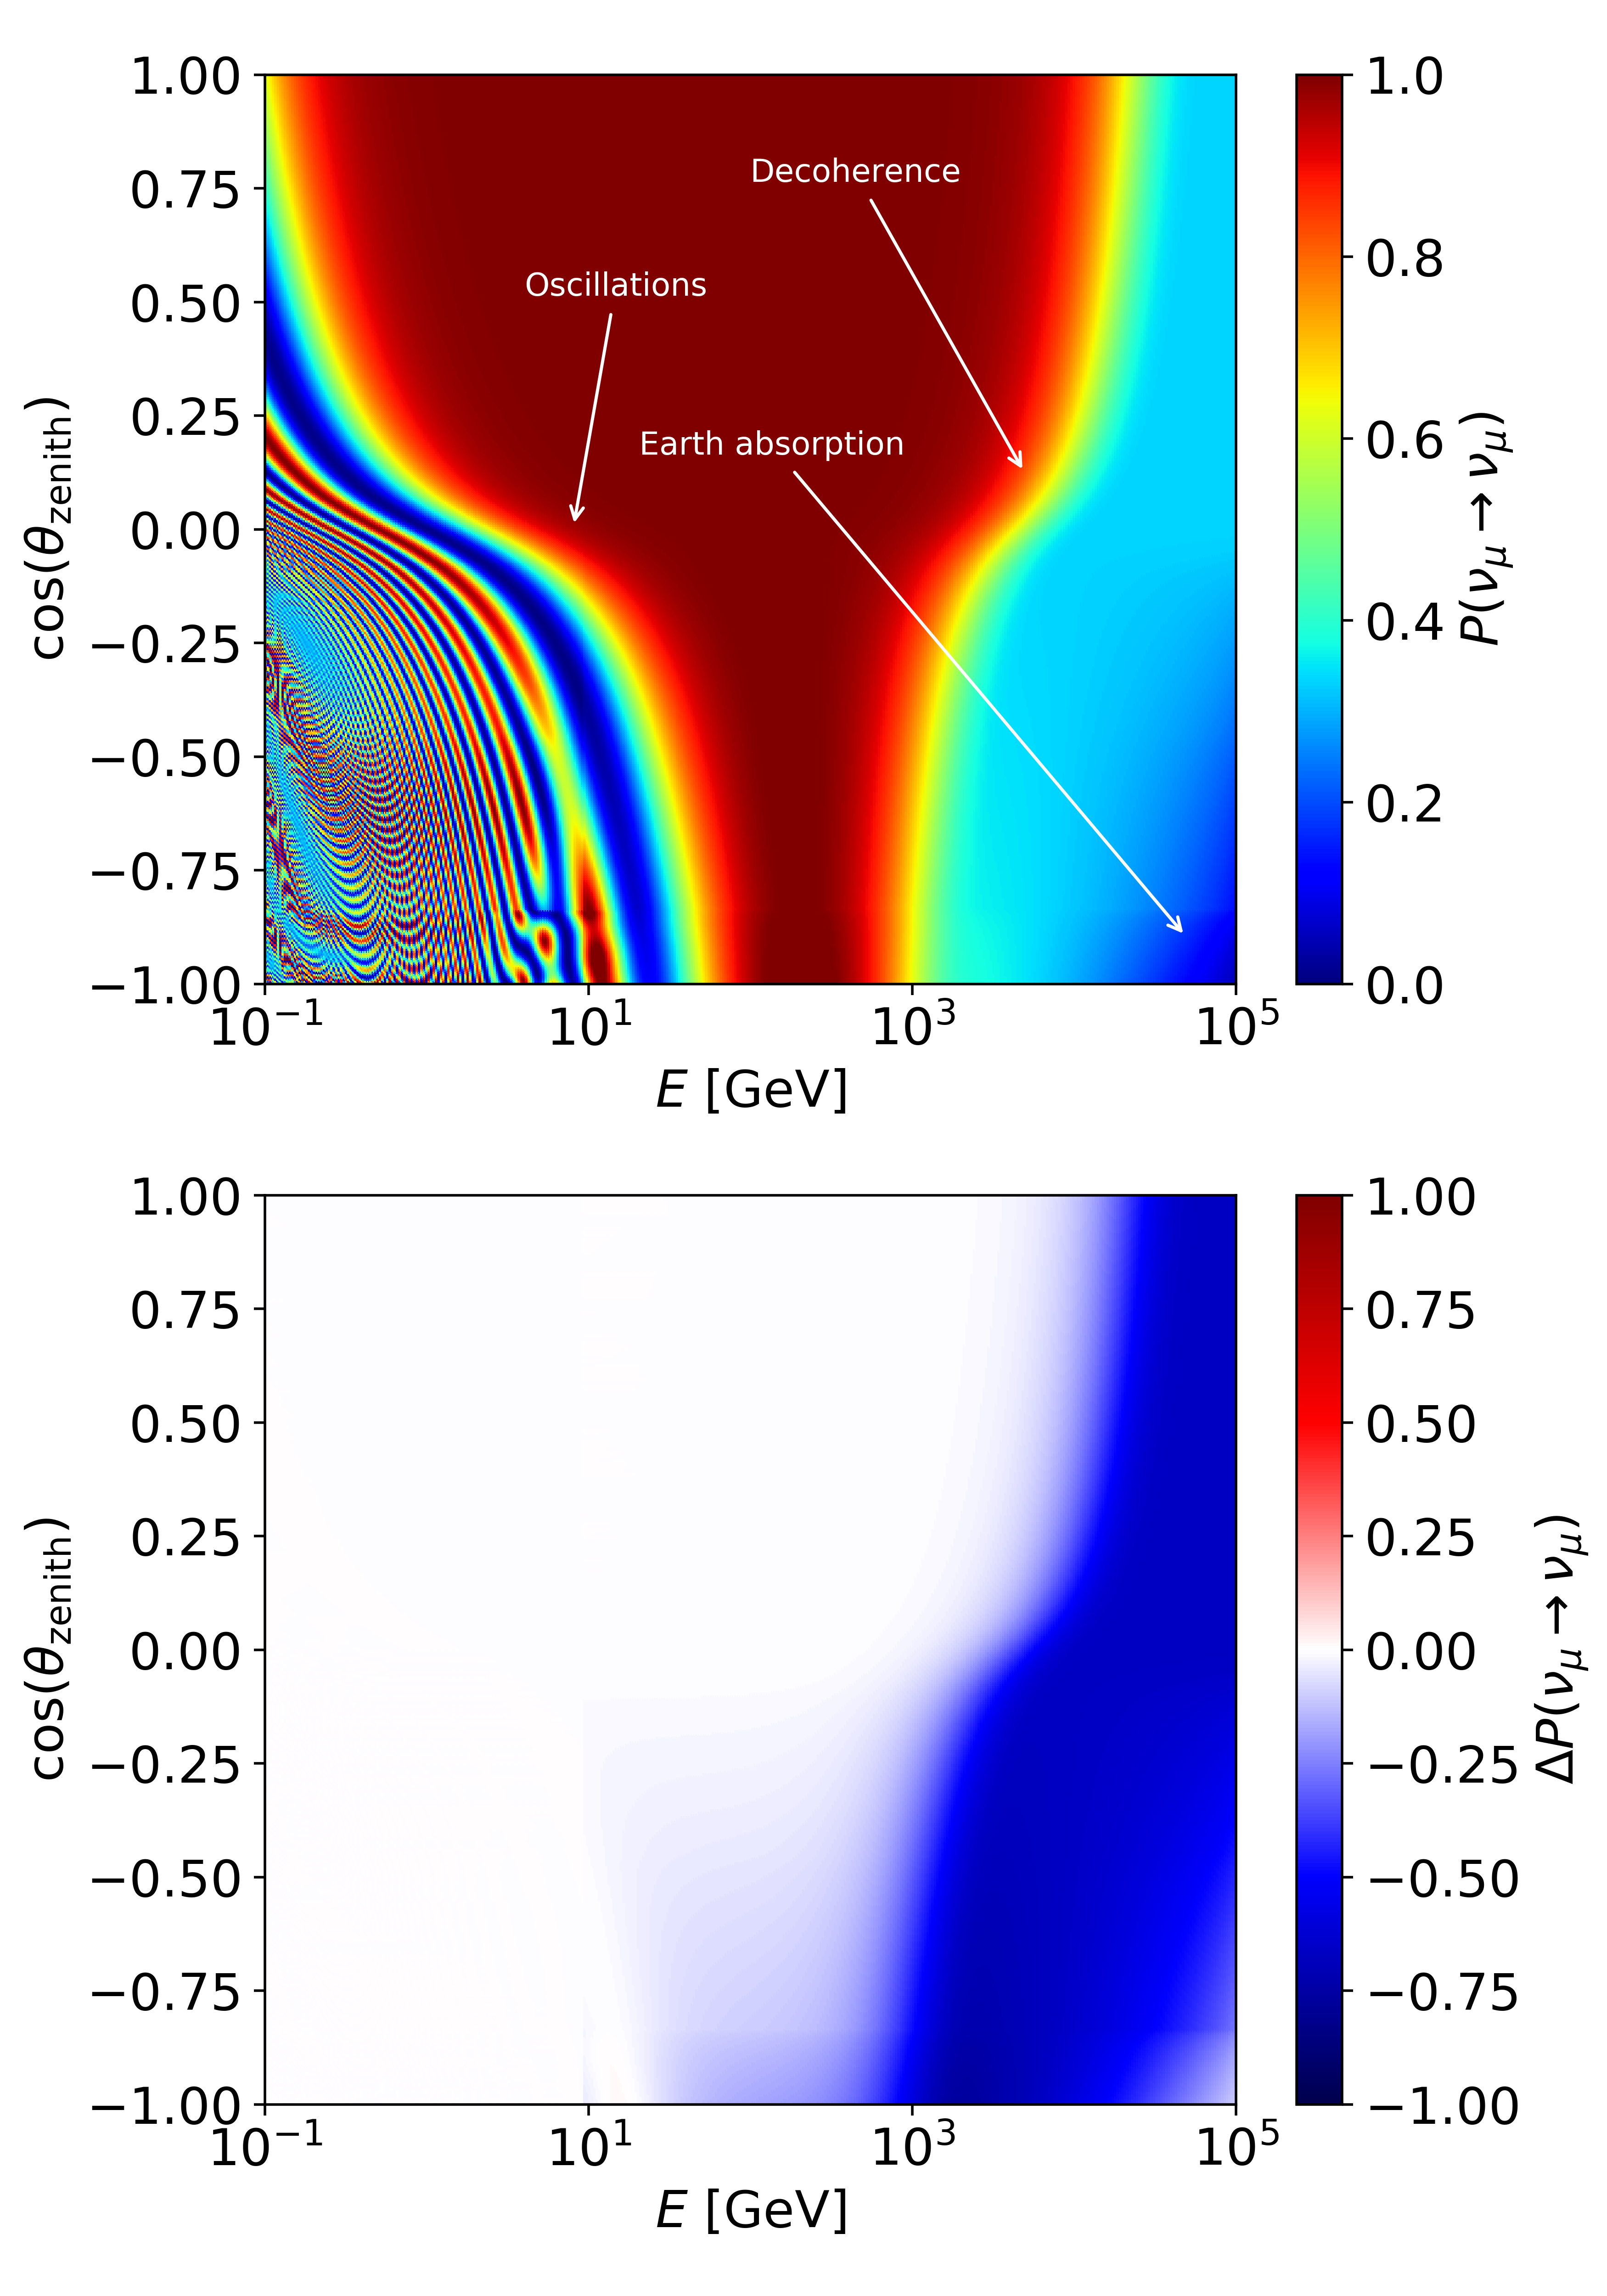
\includegraphics[trim=0.0cm 12.7cm 0.cm 0.2cm, clip=true, width=1.\linewidth]{images/atmo_oscillogram_randomize_flavor_n2_matter.png}
    \caption{}
    \end{subfigure}
    \caption{Modified atmospheric neutrino oscillations vs. neutrino energy (x axis) and arrival direction (y axis) in my $\nu$-VBH interaction decoherence models, showing (a) energy-independent and (b) $E^2$ dependent scenarios (to which accelerator experiments have far inferior sensitivity)~\cite{PhysRevD.102.115003}. Detectable features are present across a broad range of energies.}
    \label{fig:decoh_oscillograms}
\end{figure}

The event sample and simulations developed in this project will form the core of both the $CPT$-V and decoherence analyses, both of which will also utilise my existing oscillation analysis framework, modified to include the new systematic uncertainty and signal modelling. The measurements will search for distortions in the atmospheric neutrino spectrum in IceCube in 4-dimensions; reconstructed neutrino energy, arrival direction (a proxy for travel distance), flavour, and neutrino vs antineutrino (using the new methods developed in this project).

For the $CPT$-V search I will separately fit the oscillation properties (mixing angles and mass splittings) of neutrinos and antineutrinos, in particular performing the world's first test of the possibility that any deviation between these parameters is energy-dependent, motivated by the expectation that the effects of quantum gravity are suppressed below the Planck scale (using a common phenomenological energy-dependence parameterisation with the decoherence search). The measurement will fit the properties of this energy-dependence, including the energy scale of the new physics producing the $CPT$-V \todo{Equation? State that expect Planck scale}. These measurements of neutrino oscillations are an order of magnitude or more higher than in energy than any previous $CPT$-V search and with far higher statistics, giving unprecedented sensitivity to energy-suppressed effects.

\todo{Integrate this sentence:} The energy-suppressed $CPT$-V I will search for is an excellent candidate to explain this, as these effects would have been strong in the high temperatures of the early Universe when (anti)matter was forming~\cite{Mavromatos:2017cxr, hep-ph/9809542, Ellis:2013gca}.

\todo{IceCueb now more sensitive osc measurements under my leadership}

\textbf{Risk/Gain:} The $CPT$-V measurement is made possible by the pioneering (anti)neutrino separation techniques developed in this project, and thus this great opportunity to test energy-suppressed $CPT$-V is strongly contingent on the successful development of these techniques. A delay to the installation of the IceCube Upgrade would also affect this result, but the timeline is such that even a delay of one year would still yield substantial statistics for the measurement.

The signal of neutrino decoherence in IceCube is the (energy-dependent) damping of neutrino oscillations over distance, and I will test a range of decoherence models (a number of which I developed), including $\nu$-VBH interactions (see Fig. \ref{fig:decoh_oscillograms}) and lightcone fluctuations, fitting the underlying model parameters. This work will yield the \textbf{first ever measurements}\todo{Not really first due to LBL paper?} of the $\nu$-VBH interaction mean free path (in turn constraining how numerous VBHs are and their interaction cross section with neutrinos), the size of the space-time fluctuations experienced by neutrinos, and the intrinsic variability of neutrino velocity (so-called \textit{stochastic Lorentz invariance violation}~\cite{Vasileiou2015, Amelino-Camelia:2016fuh}). I will also test neutrino decay scenarios since it shares common damping features to the decoherence signals I am probing, increasing the physics output of this work. I will also perform a model-independent search (the first of its kind), fitting the matrix elements of a generalised \textit{decoherence operator}, expressed in the mathematical framework of \textit{open quantum systems} (REFS), and the energy-dependence, giving sensitivity to virtually any possible source of neutrino decoherence. 

\textbf{Risk/Gain:} The development of an event sample spanning six orders of magnitude in energy in this project is a major (challenge), but will yield unprecedented sensitivity to the broadest range of decoherence scenarios ever tested, particularly if strongly energy-suppressed (as expected for quantu gravity).

% \textbf{Risk/Gain:} This generalised decoherence search will feature many free parameters in the fit, a major computational challenge for the frequentist \textit{minimisation} algorithms used in most oscillation analyses. Should this prove untenable, I will instead employ Bayesian Markov Chain Monte Carlo (MCMC) methods which have been shown to perform better in many parameter fits. This will require a significant time investment implementing these methods in my analysis software framework\todo{Probably drop this - boring}.

A frequent prediction in quantum gravity phenomenology is that $CPT$-V manifests as differences between neutrino and antineutrino decoherence effects~\cite{Mavromatos_2009, Barenboim:2004wu, Carrasco:2018sca, Buoninfante:2020iyr, Capolupo:2020myw}, which has never been experimentally tested. I will exploit this opportune synergy in this project  to perform the world's first search for $CPT$-V decoherence in this project, testing $CPT$-V decoherence operators~\cite{Carrasco:2018sca, Buoninfante:2020iyr, Capolupo:2020myw} and giving the prospect of detecting $CPT$-V even if neutrino-antineutrino mixing angle and mass splitting differences prove immeasurably small.

This work will be by far the most sensitive and comprehensive search for energy-suppressed neutrino decoherence and $CPT$-V ever performed, and crucially will achieve sensitivity to the naturally expected scale of quantum gravity effects for the $\nu$-VBH interactions models tested up to even cubic energy-suppression, guaranteeing either the first detection of quantum gravity or the rejection of a range of well motivated models. Either way these results will be invaluable in informing the theoretical development of quantum gravity, and I will seek to publish these results in the high impact journal \textit{Nature}. \\

\textbf{Integrate this:} Detecting $CPT$-V would have profound consequences even beyond the search for quantum gravity. One of the biggest questions in physics is why the Universe appears to almost entirely consist of matter, and not antimatter, since (in the absence of $CPT$-V or other new physics) both are expected to have been produced equally. The very fact we are even here to ponder this question is a consequence of this, since without this imbalance all matter and antimatter would have annihilated to leave a Universe devoid of stars, planets or life. 


\subsubsection{Conclusion}

TODO See Jason's \\

This project will produce genuinely game changing advances in both experimental searches for quantum gravity with neutrinos and in the technical sophistication of IceCube data analysis methods (befitting the next-generation IceCube Upgrade detector), being one of very measurements globally to achieve sensitivity to the naturally expected scale of quantum gravity effects.

TODO high E oscillation wit next-gen detector to give best sensitivity ever to quantuk gravity and matter-antimatter asymmetry
TODO Cover risk again

TODO showcasing vision, innovation, etc. Impatc of anti/nu stuff...


% % I will create a number of masters projects to further explore the opportunities of this cutting edge research, drawing on my proven track record of masters project supervision (five students, producing publications and/or key contributions to IceCube oscillation measurements). I include travel budget to allow these students gain valuable experience presenting their work at conferences. 

% There are also natural opportunities to extend the scope of this research by providing valuable opportunities for MSc students, and I foresee creating the following MSc projects:

% \noindent \textbf{[Project 1]} I have identified that the very precise measurements of muons orbiting in magnetic fields by the Fermilab muon g-2 experiment~\cite{Grange:2015fou} are sensitive to lightcone fluctuations. The student will model these effects to quantify the sensitivity, with a view to a full measurement in a future proposal.\\
% \noindent \textbf{[Project 2]} Analysis constraining $\nu$-VBH interactions for neutrinos travelling cosmological distances, using neutrino and gamma-ray observations from the flaring blazar TXS 0506+056~\cite{eaat1378}.\\
% % \noindent \textbf{[Project 3]} Study the potential of neutrinos produced in high energy cosmic ray interactions with the Sun's atmosphere for quantum gravity measurements, where the larger travel distances should yield stronger decoherence effects than the terrestrial atmospheric neutrinos considered here.\\
% % \noindent \textbf{[Project 3]} Investigate neutrino decoherence from Dark Matter backgrounds~\cite{1909.11271, EPJC802020}.\\
% \noindent \textbf{[Project 3]} Investigate the potential of astrophysical neutrino $CPT$-V measurements using the (anti)neutrino discrimination techniques developed in this project.
% % \noindent \textbf{[Project 4]} Develop an atmospheric muon sideband in Analysis A to constrain the dominant systematic uncertainties (cosmic ray air shower modelling and ice optical properties), increasing sensitivity.


\todo{Outlook?}

% ------------------------------------------------------------------------------
% ------------------------------------------------------------------------------
% ------------------------------------------------------------------------------

\newpage

%\begin{multicols}{2}
\bibliography{references}
%\end{multicols}


%%%%%%%%%%%%%%%%%%%%%%%%%%%%%%%%%%%%%%%%%%%%%%%%%%%%%%%%%%
% CV
%%%%%%%%%%%%%%%%%%%%%%%%%%%%%%%%%%%%%%%%%%%%%%%%%%%%%%%%%%
\newpage

\section{Curriculum Vitae}

% \chead{B1 - Curriculum Vitae}

\textbf{PERSONAL INFORMATION ~~\hrulefill}\smallskip\\
Name: Thomas Simon Stuttard \\
Date of Birth: 3rd December 1985\\
Nationality: British

%=======================================================================
%=======================================================================
% Education
%
\textbf{EDUCATION ~~\hrulefill}\smallskip\\
%
{\bf PhD in Physics} \hfill {\em 2017} \\ 
University College London, United Kingdom // Fermilab muon g-2 experiment

{\bf MSci in Physics and Astrophysics, 1st class} \hfill {\em 2009} \\ 
University of Bristol, United Kingdom \\
Awarded the Masters thesis prize (International Linear Collider, ILC)

% \begin{tabular*}{\textwidth}%
%   {@{\extracolsep{\fill}}lcr}
%   2017 & PhD in Physics \\
%   & University College London, UK \\
%   & Supervisor: Professor Mark Lancaster \\
%   %\multicolumn{3}{l}{- Advisor: Prof. Jenny Thomas} \smallskip
%   \\
%   University of Minnesota-Duluth & \bf{M.S.}, Physics & 2004 \\
%   %\multicolumn{3}{l}{- Advisor: Prof. Alec Habig} \smallskip
%   \\ 
%   Rensselaer Polytechnic Institute & \bf{B.S.}, Physics & 2002 \\
% \end{tabular*}
% ~\smallskip \\
% \indent
%
%== End Education block
%
%=======================================================================
%=======================================================================
\textbf{CURRENT POSITION ~~\hrulefill}\smallskip\\
%
{\bf Assistant professor} \hfill {\em 2020 - present} \\ 
Niels Bohr Institute, Denmark // IceCube

\textbf{PREVIOUS POSITIONS ~~\hrulefill}\smallskip\\
%
{\bf Postdoc} \hfill {\em 2016 - 2020} \\ 
Niels Bohr Institute, Denmark // IceCube

{\bf Simulation Engineer} \hfill {\em 2009 - 2013} \\ 
Airbus Space (formerly EADS Astrium), United Kingdom \& France\\
European Space Agency ExoMars Rover, Solar Orbiter and GAIA missions. Project leader of Solar Orbiter platform and payload simulations (6 engineers across 3 countries). \\
This industry position was prior to my PhD and the start of my academic career. 

%=======================================================================
%=======================================================================
\textbf{SUPERVISION OF GRADUATE STUDENTS AND POSTDOCTORAL FELLOWS ~~\hrulefill}\smallskip\\
%
{\bf MSc} \hfill {\em 2017 - present} \\
5 students (co-supervisor), Niels Bohr Institute, Denmark
% Kasper Pedersen (ongoing), Jonathan Jegstrup (ongoing), Thomas Halberg (2019), Ida Storehaug (2019), Mikkel Jensen (2089)

%=======================================================================
%=======================================================================
\textbf{ORGANISATION OF SCIENTIFIC MEETINGS ~~\hrulefill}\smallskip\\
%
{\bf International PhD Summer School on Neutrinos} \hfill {\em 2021} \\ 
  Niels Bohr Institute, Denmark - Co-organiser
  
{\bf Particle Physics with Neutrino Telescopes (PPNT)} \hfill {\em 2019} \\ 
  Uppsala University, Sweden (39 participants) - Session chair
  
{\bf IceCube Upgrade design workshop} \hfill {\em 2019} \\ 
  Michigan State University, US (35 participants) - Session organiser

{\bf IceCube Upgrade simulation and reconstruction workshop} \hfill {\em 2018} \\ 
  Niels Bohr Institute, Denmark (19 participants) - Primary workshop organiser

{\bf IceCube oscillation analysis software code sprint} \hfill {\em 2018} \\ 
  Niels Bohr Institute, Denmark (5 participants) - Primary workshop organiser

{\bf Niels Bohr Institute experimental neutrino physics journal club} \hfill {\em 2017 - present} \\ 
Primary organiser of bi-weekly event with $\sim20$ attendees, bridging gap between theorists and experimentalists.

\todo{Collab meeting, osc meetings}
  
%=======================================================================
%=======================================================================
\textbf{INSTITUTIONAL RESPONSIBILITIES ~~\hrulefill}\smallskip\\
%
{\bf IceCube oscillation physics working group co-convener} \hfill {\em 2018 - present} \\ 
Leading oscillations working group in IceCube ($\sim$30 scientists in 11 institutes - US, Canada, Germany, UK and Denmark), including Beyond Standard Model (BSM) oscillations. Responsible for all oscillation analyses and publications, weekly conference calls and twice-annual collaboration meetings in Europe, US and Japan. 

{\bf IceCube Upgrade Simulation Manager} \hfill {\em 2018 - present} \\ 
Managing collaboration-wide simulation efforts for the IceCube Upgrade. Named responsible person to the US National Science Foundation for the simulation of all in ice detector and calibration devices. Also coordinating reconstruction, data processing and analysis efforts during the detector development phase.

{\bf IceCube Upgrade Technology Board} \hfill {\em 2018 - present} \\ 
Member of board overseeing technology requirements, development, procurement, quality control and commissioning for the IceCube Upgrade.

{\bf IceCube Coordination Committee} \hfill {\em 2018 - present} \\ 
Member of committee coordinating IceCube human and computing resources, software priorities, and connections between technical and science working groups.

{\bf European Committee for Future Accelerators (ECFA) } \hfill {\em 2019} \\ 
Early career scientist representative for Denmark.

{\bf Snowmass 2021 } \hfill {\em 2020 - present} \\ 
IceCube point of contact for neutrino oscillation physics for US Particle Physics Community Planning.

%=======================================================================
%=======================================================================
\textbf{REVIEWING ACTIVITIES ~~\hrulefill}\smallskip\\
%
{\bf COST Action CA18108 quantum gravity phenomenology reviewer  } \hfill {\em 2021} \\ 
Invited contributor to pan-European review, primary author for topic of neutrino decoherence.

\todo{All IceCube osc analyses}

%=======================================================================
%=======================================================================
\textbf{MAJOR COLLABORATIONS ~~\hrulefill}\smallskip\\
%
{\bf IceCube collaboration} \\ 
Member of the 300-person IceCube collaboration across Europe, US and Asia.

{\bf COST Action CA18108: Quantum gravity phenomenology in the multi-messenger approach} \\ 
Member of an international collaboration seeking evidence of quantum gravity.

{\bf Fermilab muon g-2 collaboration} \\ 
Member of the 200-person international collaboration searching for new physics with precision muon measurements.


\todo{Funding applications page - see Jason template}

%
%%%%%%%%%%%%%%%%%%%%%%%%%%%%%%%%%%%%%%%%%%%%%%%%%%%%%%%%%%
% Funding ID
%%%%%%%%%%%%%%%%%%%%%%%%%%%%%%%%%%%%%%%%%%%%%%%%%%%%%%%%%%
\newpage 

\lhead[\it Koskinen]{\it Koskinen}
\chead{B1 - Funding ID}
\rhead{NuUnity}


%~\vspace{2cm}

\centerline{ {\textit{\textbf{ Appendix: All on-going and submitted grants and funding of the PI (Funding ID)}}
}} \smallskip
\centerline{ \it \underline{Mandatory information} (does not count towards page limits)
}\smallskip

~\vspace{2cm}

{\bf On-going Grants}
\begin{table}[h]
\centering
\begin{tabularx}{1\textwidth}{|C{0.125\textwidth}|C{0.125\textwidth}|C{0.0817\textwidth}|C{0.125\textwidth}|C{0.125\textwidth}|C{0.26\textwidth}|}
\hline
\rowcolor[gray]{0.85} \it Project~Title & \it Funding Source & \it Amount (Euros) & \it Period & \it Role of the PI & \it Relation to current ERC Proposal\\
\hline
Neutrinos on Ice & Villum Foundation & 659\,134& Mar.~2016 --- Dec.~2020 & Principal Investigator & Analysis software preparation for joint DeepCore \& IceCube Upgrade data \\
\hline
NuFront: Neutrinos at the Physics Frontier& Carlsberg Foundation & 601\,989& Mar.~2020 --- Feb.~2023 & Principal Investigator & Focuses on $\nutau$ appearance measurement in geometry optimization for the IceCube Upgrade and bridging the gap between IceCube-DeepCore data taking and the start of the IceCube Upgrade data taking \\
\hline
\end{tabularx}
\end{table}

~\vspace{2cm}


{\bf Grant Applications}
\begin{table}[h]
\centering
\begin{tabularx}{1\textwidth}{|C{0.125\textwidth}|C{0.125\textwidth}|C{0.0817\textwidth}|C{0.125\textwidth}|C{0.125\textwidth}|C{0.26\textwidth}|}
\hline
\rowcolor[gray]{0.85} \it  Project Title & \it Funding Source & \it Amount (Euros) & \it Period & \it Role of the PI & \it Relation to current ERC Proposal\\
\hline
None at the time of submission & $~~~~~~~~~~~~~~~~~~~$ & & & & \\
\hline
\end{tabularx}
\end{table}

%%%%%%%%%%%%%%%%%%%%%%%%%%%%%%%%%%%%%%%%%%%%%%%%%%%%%%%%%%
% Track Record
%%%%%%%%%%%%%%%%%%%%%%%%%%%%%%%%%%%%%%%%%%%%%%%%%%%%%%%%%%

\newpage

\subsection{Track record}

\todo{Publications score}

\textbf{From instructions:} Section c: Early achievements track-record (max. 2 pages) should list your important achievements,
including your most important publications27 (up to five for Starting Grant and up to ten for
Consolidator Grant) highlighting those as main author and/or without the co-authorship of your PhD
supervisor. The publications should be properly referenced, including all authors in the published
order (Please see section 1.1 on Research integrity). Field relevant bibliometric indicators as well as
research monographs and any translations thereof may also be included. If applicable include:
granted patent(s); invited presentations to internationally established conferences and/or
international advanced schools; Prizes/Awards/Academy memberships etc. 

%=======================================================================
%=======================================================================
\textbf{INVITED CONFERENCE TALKS ~~\hrulefill}\smallskip\\
%
{\it Latest results from IceCube} \hfill {\em Invited talk} \\ 
 Moriond Electroweak 2021 - France (Virtual) - 2021
 
 {\it GeV-scale BSM physics with IceCube/DeepCore and the IceCube Upgrade} \hfill {\em Invited talk} \\ 
%  Workshop on Interplay of Neutrino and Dark matter Experiments and Exotic Searches 2021 - Korea (Virtual)l - 2021
 INDEEES 2021 - South Korea (Virtual) - 2021

 {\it IceCube: oscillations and BSM} \hfill {\em Invited talk} \\ 
 XIX International Workshop on Neutrino Telescopes - Germany (Virtual) - 2021
 
{\it Neutrino oscillation with IceCube-DeepCore and the IceCube Upgrade} \hfill {\em Invited talk} \\ 
 Snowmass 2021 - US - 2020
 
% {\it Environmentally-induced neutrino decoherence with IceCube/DeepCore, and neutrino oscillation physics prospects with the IceCube Upgrade} \hfill {\em Invited talk} \\ 
{\it Neutrino decoherence with IceCube and neutrino oscillations with the IceCube Upgrade} \hfill {\em Invited talk} \\ 
 Particle Physics with Neutrino Telescopes (PPNT) - Sweden - 2019
 
{\it Tau neutrino appearance and the PMNS matrix with IceCube and the IceCube Upgrade} \hfill {\em Invited talk} \\ 
 21st International Workshop on Neutrinos from Accelerators (NuFact) - South Korea - 2019

% {\it Probing environmentally-induced neutrino decoherence with IceCube} \hfill {\em Contributed talk} \\ 
%  Annual Meeting of the Danish Physical Society (Dansk Fysisk Selskab) - Denmark - 2019

{\it Latest astrophysical and particle physics results and future prospects from IceCube} \hfill {\em Invited talk} \\ 
 International Conference on Particle Physics and Astrophysics (ICPPA) - Russia - 2018

{\it Measurement of Atmospheric Neutrino Oscillations with IceCube and DeepCore} \hfill {\em Invited talk} \\ 
 Advanced Workshop on Physics of Atmospheric Neutrinos (PANE) - Italy - 2018
 
 
 

\lhead[\it Koskinen]{\it Koskinen}
\chead{B1 - Track Record}
\rhead{NuUnity}

Through my leadership roles in the IceCube collaboration and central impact regarding $\nu_\tau$ appearance analyses, I have been grateful to be the official IceCube speaker at major conferences and workshops. Further evidence of my standing within the field are $25+$ personal invitations for seminars and colloquia at universities (Harvard, MIT, Columbia, Oxford, etc.) and National Laboratories (Fermilab, Lawrence Berkeley, and Brookhaven), as well as being an invited lecturer at $3$ weeklong Ph.D.\@ schools. I am also committed to science outreach and my group hosts events at \href{https://www.kulturnatten.dk/da/Kulturnatten}{KBH Kulturnatten}, day-long workshops for high school students at the NBI, walking tours at the 2019 BLOOM festival and interactive museum shows for \href{https://samtidskunst.dk/sites/default/files/press/pressemeddelelse_uk_weak_force.pdf}{\texttt{[WEAK] FORCE}} by Lea Porsager, evening lectures for \href{https://nbia.nbi.ku.dk/calendar/past/public/}{Folkeuniversitet i K{\o}benhavn}, and much more.

\noindent
\textbf{SELECTED PUBLICATIONS ~~\hrulefill}\\ 
All statistics are from \texttt{inspire-hep} and include $198$ ($148$) total published (citable) papers with $19941$ ($18441$) citations, for an h-index of $73$($71$).
%
\noindent
\begin{etaremune}[topsep=0pt,itemsep=1.0pt,partopsep=0pt,parsep=0pt]
\itemsep 1pt
%
\item{C.\@ Pérez de los Heros (Editor), ``Probing Particle Physics With Neutrino Telescopes". Book. World Scientific (2019).}
\begin{itemize}
\item{I wrote the chapter on `Standard Neutrino Oscillations' for a book targeting Ph.D.\@ students in particle and astroparticle physics.\smallskip}
\end{itemize}
%
\item{M.\@ G.\@ Aartsen {\it et al.\@} [IceCube Collaboration], ``Measurement of Atmospheric Tau Neutrino Appearance with IceCube DeepCore". Phys.\ Rev.\ D{\bf99} 032007 (2019). \hfill [{\tt 16~citations}]}
\begin{itemize}
\item{This is the world leading result on nutau appearance, and constraints on non-unitarity in neutrino oscillations. The main analysis came for my group and was led by my Ph.D.\@ student Michael Larson.\smallskip}
\end{itemize}
%
\item{M.\@ G.\@ Aartsen {\it et al.\@} [IceCube Collaboration], ``Search for neutrinos from dark matter self-annihilations in the  center of the Milky Way with 3 years of IceCube/DeepCore". Eur.\ Phys.\ J.\ C{\bf77}, 627 (2017). \hfill [{\tt 67~citations}]}
\begin{itemize}
\item{This is the analysis and world leading results on dark matter self-annihilation to neutrinos from my Ph.D. student Morten Medici.\smallskip}
\end{itemize}
%
\item{R.~Abbasi {\it et al.}~~[IceCube Collaboration], ``The Design and Performance of IceCube DeepCore,''  Astropart.\ Phys.\  {\bf 35}, 615 (2012).\hfill[{\tt 279~citations}]}
\begin{itemize}
\item{I was one of the writers and editors, generated the simulation data sets, produced the trigger and effective volume/area performance plots, and prepared all plots and figures.\smallskip}
\end{itemize}
%
\item{ D.~J.~Koskinen, ``IceCube-DeepCore-PINGU: Fundamental neutrino and dark matter physics at the South Pole," Mod.\ Phys.\ Lett.\ A{\bf 26}, 2899 (2011). \hfill[{\tt 61 citations}]}
\begin{itemize}
\item{\textbf{Single author paper which is the first published account of PINGU, and is the precursor to the `IceCube Upgrade'.}\smallskip}
\end{itemize}

%\item{$^*$D.~G.~Michael {\it et al.}~~[MINOS Collaboration], ``Observation of muon neutrino disappearance with the MINOS detectors and the NuMI neutrino beam,'' Phys.\ Rev.\ Lett.\  {\bf 97}, 191801 (2006).~~~~~~~~~~~~~  \hfill [{\tt 596 citations}]}
%\begin{itemize}
%\item{I contributed to the treatment of systematic uncertainties.\\}
%\end{itemize}
\end{etaremune}

%
% Name and address
%
%~\medskip
%~
%\centerline{ \large \textbf{Track Record - David Jason Koskinen}} \smallskip \\
%
%
%=======================================================================
%=======================================================================
%
%
%\textbf{PROFESSIONAL ACTIVITIES ~~\hrulefill} \smallskip \\ 
%
%$\bullet$ Lecturer at the 2015 \textit{Nordic Winter School on Cosmology and Particle Physics}\smallskip \\
%
%$\bullet$ Board member of the \textit{Discovery Centre for Particle Physics} at the Niels Bohr Institute\smallskip \\
%
%$\bullet$ Lecturer at the 2014 Niels Bohr International Academy Ph.D. school \textit{Neutrinos Underground and in the Heavens}\smallskip \\
%
%$\bullet$ Creator and organizer of the 2014 \textit{Astroparticle Neutrino Physics in Antarctica Workshop} hosted at the Niels Bohr Institute\smallskip \\
%
%== End Committee block
%
%=======================================================================
%=======================================================================
%
% Presentations
%
%\newpage
%
\noindent
\textbf{INVITED CONFERENCES \& WORKSHOPS ~~\hrulefill}
%
\begin{multicols}{2}
\begin{etaremune}[topsep=0pt,itemsep=4pt,partopsep=0pt,parsep=0pt]
\itemsep 3.5pt
%\setlength{\itemindent}{0em}
%
\item{\textit{IceCube - Particle Physics and Astrophysics on Ice} - 
\href{https://indico.nbi.ku.dk/event/1259/}{Nordic Conference on Particle Physics}~~-~~Skeikampen, Norway~~-~~January 3, 2020.}
%
%
\item{\textit{IceCube and Gen2: Atmospheric and Oscillation Results and Status} \\ 
\href{https://www.iopconferences.org/iop/frontend/reg/thome.csp?pageID=583922&eventID=1058&traceRedir=2&eventID=1058}{Next Generation Nucleon Decay and Neutrino Detectors (NNN17)} - University of Warwick - October 27, 2017.}
%
\item{\textit{Neutrino Physics with the PINGU Extension to IceCube}  - 
 \href{https://indico.cern.ch/event/469963/}{TeV Particle Astrophysics 2016 (TeVPA)} - CERN - September 12, 2016.}
%
%
 \item{\textit{Atmospheric neutrino results from IceCube/DeepCore and plans for PINGU} \\
 \href{http://neutrino2016.iopconfs.org/home}{The XXVII International Conference on Neutrino Physics and Astrophysics (Neutrino 2016)}~~-~~Imperial College London~~-~~July 6, 2016.}
%
\item{\textit{Neutrino Oscillation and Resolving the Neutrino Mass Ordering} \\
\href{http://indico.cern.ch/event/344173/overview}{ICNFP2015: International Conference on New Frontiers in Physics}~~-~~Kolymbari, Greece~~-~~August 29, 2015.}
 %
\item{\textit{Future Atmospheric Neutrino Experiments} -
\href{https://indico.ph.qmul.ac.uk/indico/conferenceDisplay.py?confId=22}{NuPhys2014: Prospects in Neutrino Physics} - Queen Mary University of London - December 16, 2014.}
%
\item{\textit{IceCube Results and PINGU Perspectives} - 
\href{http://www.ba.infn.it/~now/now2014/web-content/index.html}{Neutrino Oscillation Workshop} - Conca Specchiulla, Italy - September 12, 2014.}
%
\item{\textit{Results from IceCube and Prospects for PINGU} - 
\href{http://pprc.qmul.ac.uk/research/ipa2014}{Interplay of Particle and Astroparticle Physics} - Queen Mary University of London - August 19, 2014.}
%
\item{\textit{Dark Matter Searches and Astrophysical Neutrinos in IceCube} - 
\href{http://cp3-origins.dk/events/meetings/mass2014}{Origin of Mass 2014} - CP$^3$ Origins - May 22, 2014.}
%
\item{\textit{PINGU: Resolving the Neutrino Mass Hierarchy at the South Pole} - 
\href{https://indico.cern.ch/event/224351/}{New Directions in Neutrino Physics} - Aspen Center for Physics  - February 7, 2013.}
%
\item{ \textit{PINGU and O(1) GeV cross-sections} - 
\href{http://www.pitt.edu/~vipres/program_nu_flux.html}{Flux Measurement and Determination in the Intensity Frontier Era Neutrino Beams} - University of Pittsburgh - December 7, 2012.}
%
\item{\textit{IceCube, DeepCore and PINGU} - 
\href{http://conferences.fnal.gov/nnn12/}{Next Generation Nucleon Decay and Neutrino Detectors (NNN12)} - Fermilab - October 5, 2012.}
%
\item{ \textit{IceCube-DeepCore} - 
\href{http://alexfriedland.com/info11/}{Implications of Neutrino flavour Oscillations (INFO11)} - Santa Fe, New Mexico - June 7, 2011.}
%
\item{\textit{IceCube Neutrino Telescope} - 
\href{http://www.phy.uct.ac.za/conf/Win11/}{23$^{rd}$ International Workshop on Weak Interactions and Neutrinos (WIN'11)} - Cape Town, South Africa - January 31, 2011.}
%
\end{etaremune}
\end{multicols}

\textbf{INVITED COLLOQUIA \& SEMINARS (Selected)~~\hrulefill}
%
\begin{multicols}{2}
%\begin{etaremune}[topsep=0pt,itemsep=1.5pt,partopsep=0pt,parsep=0pt]
\begin{itemize}[topsep=0pt,itemsep=4.5pt,partopsep=0pt,parsep=0pt]
%
\item{\textit{Fundamental Neutrino Physics with a Gigaton of Ice} - University of Zurich - May 28, 2018.}
%
\item{\textit{Fundamental Neutrino Physics with a Gigaton of Ice}  - University of Oxford - May 1, 2018.}
%
\item{\textit{Neutrinos on Ice: Using IceCube to Chase a Ghost Particle} - 
Physics and Astronomy Colloquium - University of Southampton - October 10, 2014.}
%
\item{\textit{Using the IceCube Neutrino Observatory to Study Inner and Outer Space} - 
DTU Space Seminar - Technical University of Denmark - December 5, 2013.}
%
%\item{\textit{Connecting Inner and Outer Space: Astroparticle Physics Big and Small} - 
%Annual Meeting of the Danish Physical Society - University of Copenhagen - November 14, 2013.}
%
\item{ \textit{PINGU: Neutrino Hierarchy Determination at the South Pole} - 
Intensity Frontier Department Physics Discussions - Fermilab - April 11, 2013.}
%
\item{ \textit{IceCube-DeepCore-PINGU: Neutrino Physics at the South Pole} - 
Astro/Particle Seminar - University of Cincinnati - February 26, 2013.}
%
\item{ \textit{IceCube-DeepCore-PINGU: Neutrino Physics at the South Pole} - 
Institute for Nuclear and Particle Astrophysics Seminar - Lawrence Berkeley National Laboratory  - February 22, 2013.}
%
%\item{ \textit{IceCube-DeepCore-PINGU: Neutrino Physics at the South Pole} - 
%Discovery Center Seminar - Niels Bohr Institute  - February 20, 2013.}
%
%\item{ \textit{IceCube-DeepCore-PINGU: Neutrino Physics at the South Pole} - 
%Nuclear/Particle Physics Seminar - University of Colorado at Boulder - February 11, 2013.}
%
\item{\textit{IceCube-DeepCore-PINGU: Neutrino Physics at the South Pole} - 
Laboratory for Particle Physics and Cosmology Seminar - Harvard University - December 12, 2012.}
%
\item{ \textit{IceCube-DeepCore-PINGU: Neutrino Physics at the South Pole} - 
Lunchtime Seminar - Massachusetts Institute of Technology - December 11, 2012.}
%
\item{ \textit{Neutrinos at the South Pole} - 
Particle Physics Seminar - Universit\"{a}t W\"{u}rzburg - September 27, 2012.}
%
\item{ \textit{IceCube-DeepCore-PINGU: Atmospheric Neutrino Physics at the South Pole} - 
Particle Physics Seminar - Brookhaven National Laboratory - September 6, 2012.}
%
%\item{ \textit{Neutrino Oscillations at the South Pole} - 
%Nuclear/Particle/Astro/Cosmo Forum - University of Wisconsin-Madison - February 27, 2012.}
%
\item{ \textit{IceCube-DeepCore-PINGU: Fundamental Neutrino Physics at the South Pole} - 
Nuclear Physics, Astronomy, and Astrophysics Joint Seminar - Stony Brook University - December 8, 2011.}
%
%\item{ \textit{IceCube-DeepCore-PINGU: Neutrino Physics at the South Pole} - 
%Physics Seminar - University of Minnesota-Duluth - November 15, 2011.}
%
\item{ \textit{IceCube-DeepCore: The biggest little neutrino detector at the South Pole} - 
Particle Seminar - Columbia University - March 9, 2011.}
%
%\item{ \textit{DeepCore - Extending the energy reach of neutrinos in IceCube} - 
%Physics and Astronomy Colloquium - University of Alabama - December 1, 2010.}
%%
\item{ \textit{Neutrino Oscillations and (dis)appearance prospects for IceCube-DeepCore} - 
CCAPP Seminar - The Ohio State University's Center for Cosmology and AstroParticle Physics - October 19, 2010.}
%
%\item{ \textit{Initial Sterile Neutrino results from MINOS} - 
%New Perspectives - Fermilab - June 3, 2008.}
%%
%\item{ \textit{NuMI Muon Monitor Studies and First Results from the MINOS Sterile Neutrino Search} - 
%HEP Astrophysics Seminar - Pennsylvania State University - May 15, 2008.}
%%
\item{ \textit{NuMI Muon Monitor Studies and First Results from the MINOS Sterile Neutrino Search} - 
Neutrino Physics Seminar - Lawrence Berkeley National Laboratory - May 13,  2008.}
%%
%\item{ \textit{NuMI Muon Monitor Studies and First Results from the MINOS Sterile Neutrino Search} - 
%Joint HEP Neutrino Physics Seminar - University of Wisconsin-Madison - April 25, 2008.}
%%
%\end{etaremune}
\end{itemize}
\end{multicols}




\end{document}
